\documentclass{beamer}
\usepackage{tikz}
\usetikzlibrary{arrows,positioning,decorations.pathreplacing} 

\usepackage[utf8x]{inputenc}
\usepackage{amsfonts}
\usepackage{amsmath,esint}
\usepackage{graphicx}
\usepackage{multimedia}
\usepackage{amssymb}

\usepackage{epstopdf}
\usepackage{pdfpages}
\usepackage{dsfont}
\usepackage{textpos}
\usepackage[font=it]{caption}
\usepackage{bbm}
\usepackage{varwidth}
\usepackage{media9}
\usepackage{multimedia}

%\usetheme{Madrid}
\beamertemplatenavigationsymbolsempty
\setbeamertemplate{footline}[page number]{}
% \usecolortheme{wolverine}
\useinnertheme{rounded}

\definecolor{boiseBlue} {RGB}{29,72,159}
\definecolor{rojoAmor} {RGB}{171,13,4}
\definecolor{moradoAmor} {RGB}{93,8,113}
\definecolor{verdeAmor} {RGB}{98,158,31}
\definecolor{negro} {RGB}{10,10,10}
\definecolor{lgreen} {RGB}{180,210,100}
\definecolor{dblue}  {RGB}{20,66,129}
\definecolor{ddblue} {RGB}{11,36,69}
\definecolor{lred}   {RGB}{220,0,0}
\definecolor{nred}   {RGB}{224,0,0}
\definecolor{norange}{RGB}{230,120,20}
\definecolor{nyellow}{RGB}{255,221,0}
\definecolor{ngreen} {RGB}{98,158,31}
\definecolor{dgreen} {RGB}{78,138,21}
\definecolor{nblue}  {RGB}{28,130,185}
\definecolor{jblue}  {RGB}{20,50,100}

\setbeamercolor{palette primary}{fg=white,bg=black}
\setbeamercolor{frametitle}{fg=moradoAmor,bg=white}
\setbeamercolor{title page}{fg=nblue,bg=black}
\setbeamertemplate{itemize items}[circle]

\defbeamertemplate*{title page}{customized}[1][]
{
\begin{beamercolorbox}[sep=1em,wd=\textwidth,ht=8em,dp=-1em,center]{boldfont}
\usebeamerfont{title} {\center \color{norange} \Large \textbf \inserttitle}
\end{beamercolorbox}
\usebeamercolor{author}{\center \color{black}\normalsize{\insertauthor}\\[2em]}
\usebeamercolor{institute in headline}{\center \color{black}\normalsize{\insertinstitute}\\[5em]}
\usebeamercolor{date}{\center \color{black}\small{\insertdate}\\[0em]}
}


\makeatletter
    \newenvironment{withoutheadline}{
        \setbeamertemplate{headline}[default]
        \def\beamer@entrycode{\vspace*{-\headheight}}
    }{}
\makeatother

% Make lists without bullets
\newenvironment{itemizemine}{
  \begin{list}{}{
    \setlength{\leftmargin}{5em}
    \color{nred}
    \itemindent=3em
  }
}{
  \end{list}
}


\title{
Grenoble passive seismic
}
\author{{\bf Diego Domenzain}}
\institute{
\begin{tikzpicture}[remember picture, overlay] 
\node [] at (0,0) 
{
\includegraphics[height=0.7cm]{bsuwiki.png}}; 
\end{tikzpicture}
}
\date{\vspace{1em}Spring 2019}

\begin{document}

\frame{\titlepage}
%--------------------------------------------------------------------
%            outline                                                                                   
%--------------------------------------------------------------------
\frame
{
\frametitle{{\bf Outline}}
\begin{itemize}
\item Data
\item Methods
\item Implementation
\item Observations
\end{itemize}
}
%--------------------------------------------------------------------
%            data                                                                                   
%--------------------------------------------------------------------
\frame
{
\centering
{\bf Data}
}
%--------------------------------------------------------------------
%            data                                                                                   
%--------------------------------------------------------------------
\frame
{
\frametitle{{\bf Data}}
\centering
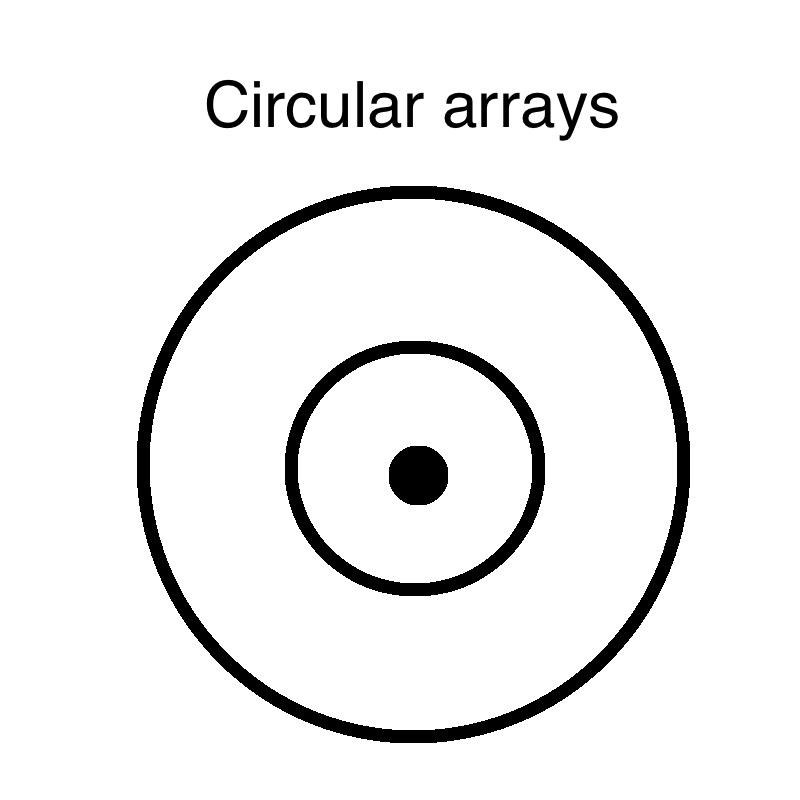
\includegraphics[width=0.7\textwidth]{../pics/idea/arrays.png}
\vfill
three of these, center in all, 3 component data
}
%--------------------------------------------------------------------
%            data                                                                                   
%--------------------------------------------------------------------
\frame
{
\centering
{\bf Methods}
}
%--------------------------------------------------------------------
%            idea                                                                                   
%--------------------------------------------------------------------
\frame
{
\frametitle{{\bf Main idea}}
\centering
seismic event $\to$ group dispersion $\to$ integral $\to$ phase dispersion
}
%--------------------------------------------------------------------
%            idea                                                                                   
%--------------------------------------------------------------------
\frame
{
\frametitle{{\bf Main idea}}
\centering
interferometry $\to$ group dispersion $\to$ integral $\to$ phase dispersion
}
%--------------------------------------------------------------------
%            idea                                                                                   
%--------------------------------------------------------------------
\frame
{
\frametitle{{\bf Inspiration}}
Campillo et al, 1996\\~\\
Shapiro et al, 1997\\~\\
Brenguier et al, 2007\\~\\
\centering
{\bf Surface-wave tomography on valleys and volcanoes from noise records and group velocities} \\~\\
(MX volcanic belt \& Piton de la Fournaise)
\vfill
\flushleft
* they use all 3 component data
}
%--------------------------------------------------------------------
%            idea                                                                                   
%--------------------------------------------------------------------
\frame
{
\frametitle{{\bf Inspiration}}
\centering
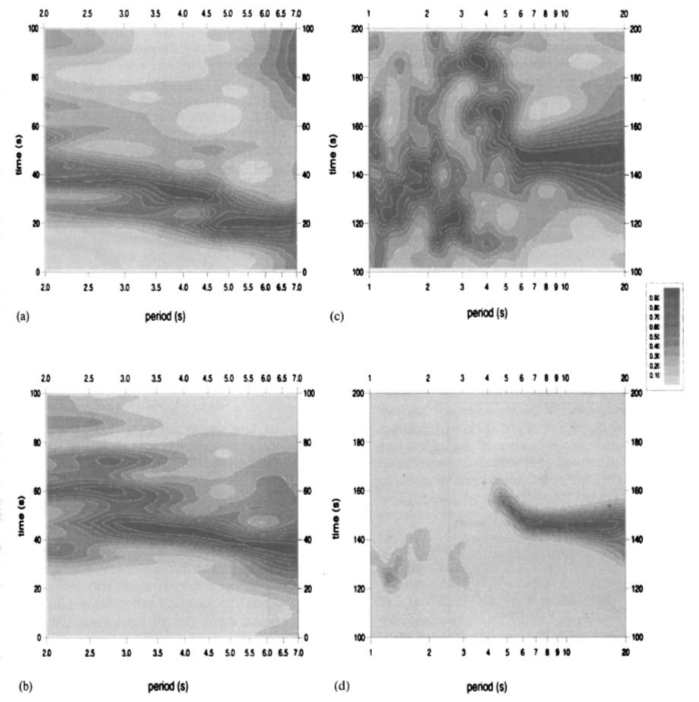
\includegraphics[width=0.7\textwidth]{../pics/idea/ftan-mex.png}
\vfill
idea is so old, it's in black and white (Shapiro et. al, 1997)
}
%--------------------------------------------------------------------
%            idea 1                                                                                   
%--------------------------------------------------------------------
\frame
{
\frametitle{{\bf Idea 1}}
\centering
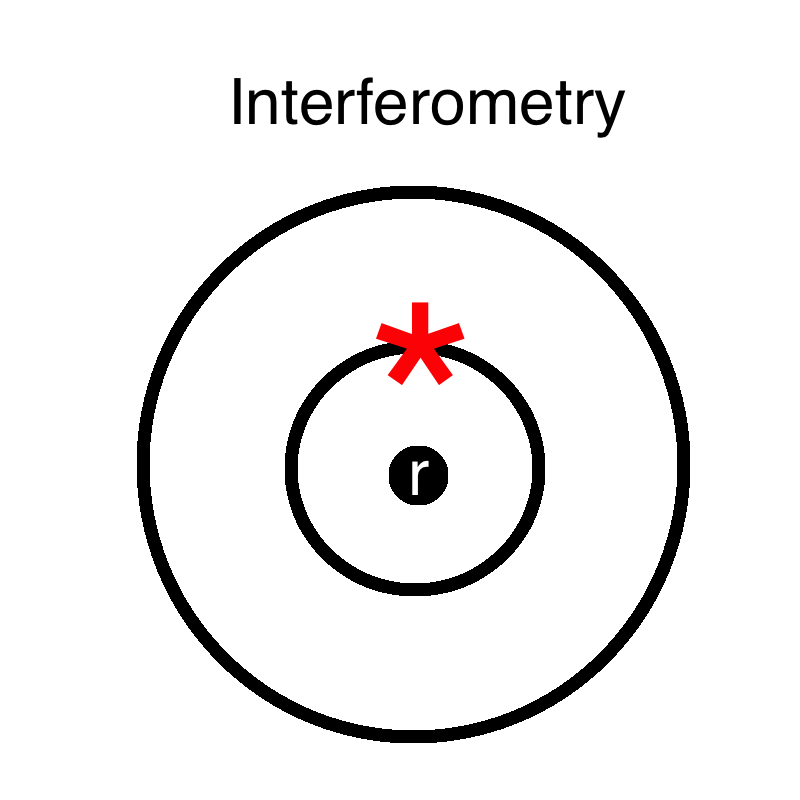
\includegraphics[width=0.7\textwidth]{../pics/idea/onyva.png}
\vfill
do many source-receiver pairs
}
%--------------------------------------------------------------------
%            idea 2                                                                               
%--------------------------------------------------------------------
\frame
{
\frametitle{{\bf Idea 2 - part 1}}
\centering
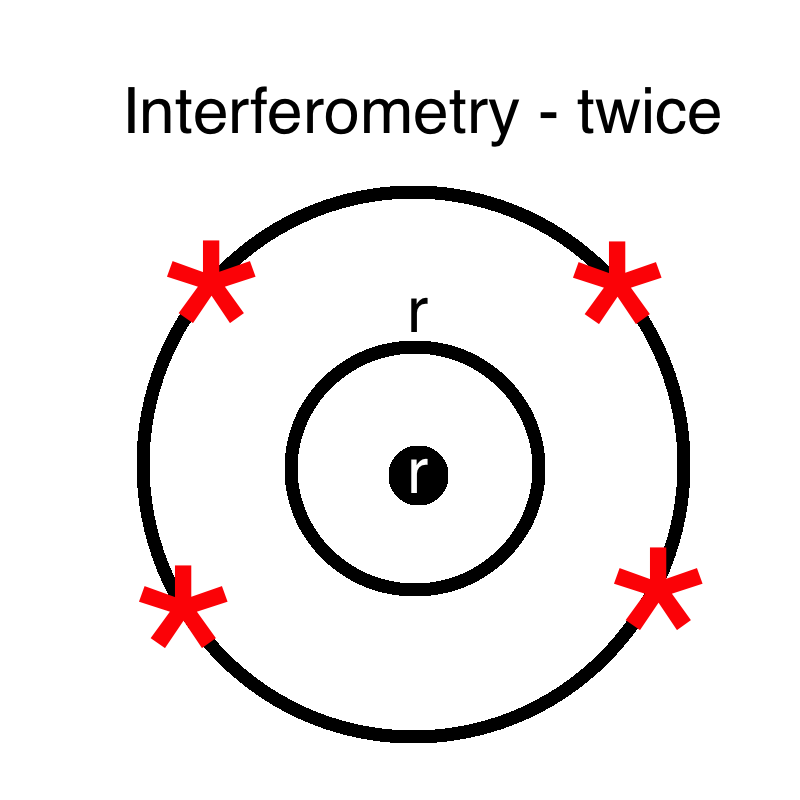
\includegraphics[width=0.7\textwidth]{../pics/idea/vamos-1.png}
\vfill
many outer virtual sources
}
%--------------------------------------------------------------------
%            idea 2                                                                                 
%--------------------------------------------------------------------
\frame
{
\frametitle{{\bf Idea 2 - part 2}}
\centering
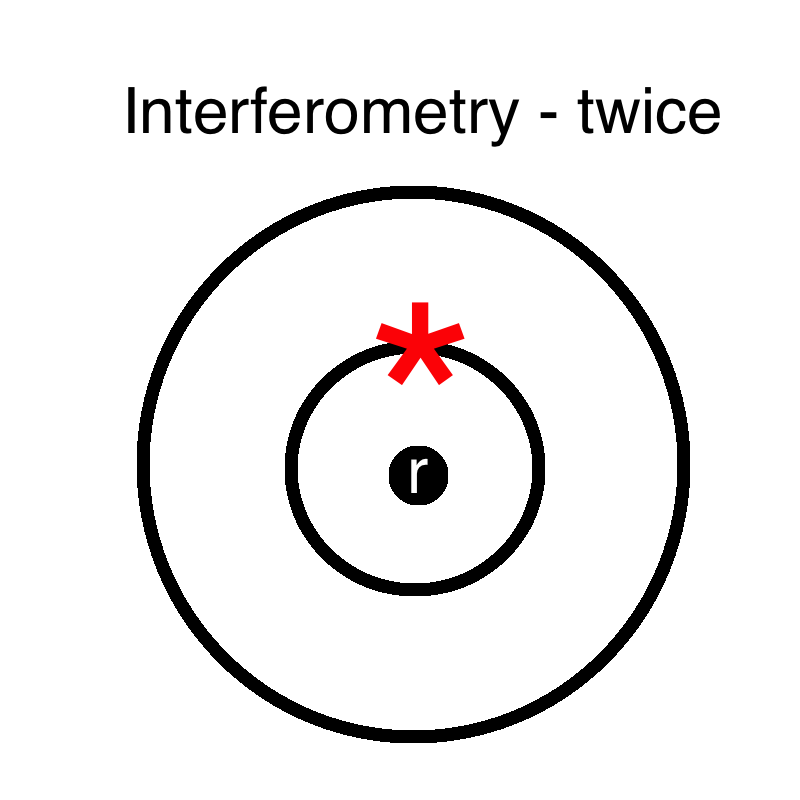
\includegraphics[width=0.7\textwidth]{../pics/idea/vamos-2.png}
\vfill
focus on one source-receiver, then do Idea 1
}
%--------------------------------------------------------------------
%            data                                                                                   
%--------------------------------------------------------------------
\frame
{
\centering
{\bf Implementation}
}
%--------------------------------------------------------------------
%            arrays                                                                                   
%--------------------------------------------------------------------
\frame
{
\frametitle{{\bf Array ``small"}}
\centering
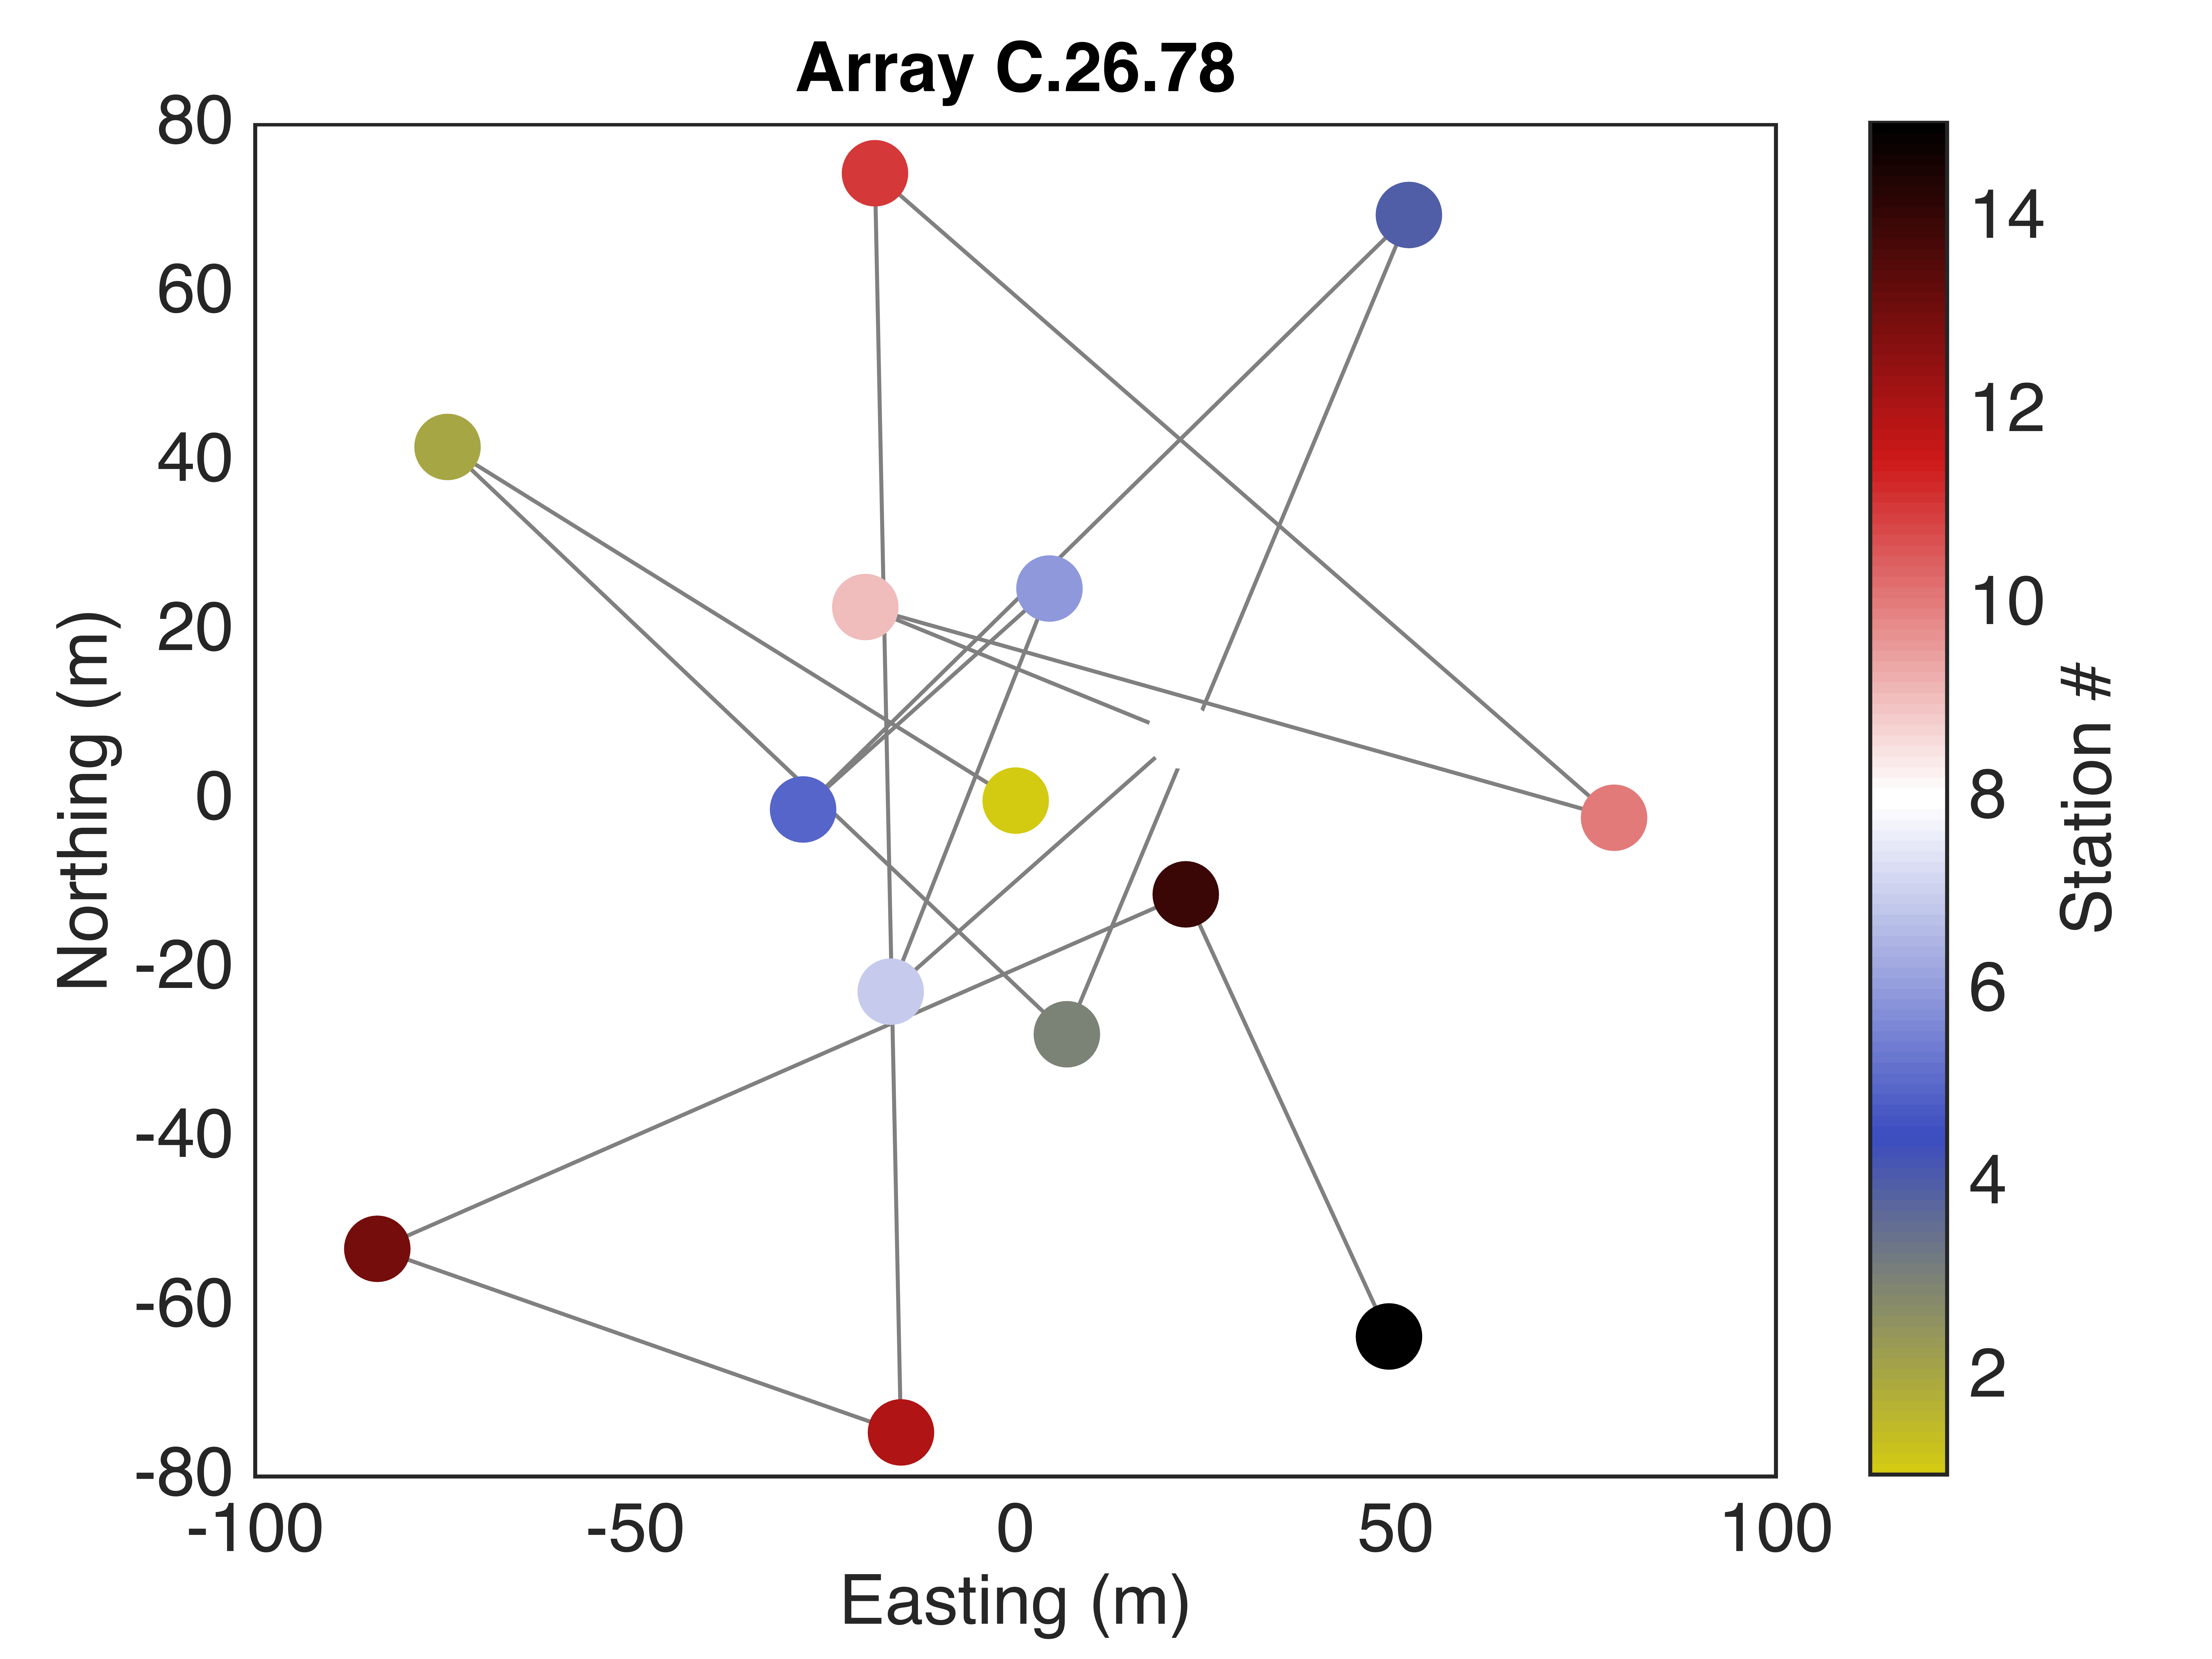
\includegraphics[width=\textwidth]{../pics/C-26-78/array.png}
}
%--------------------------------------------------------------------
%            arrays                                                                                   
%--------------------------------------------------------------------
\frame
{
\frametitle{{\bf Array ``medium"}}
\centering
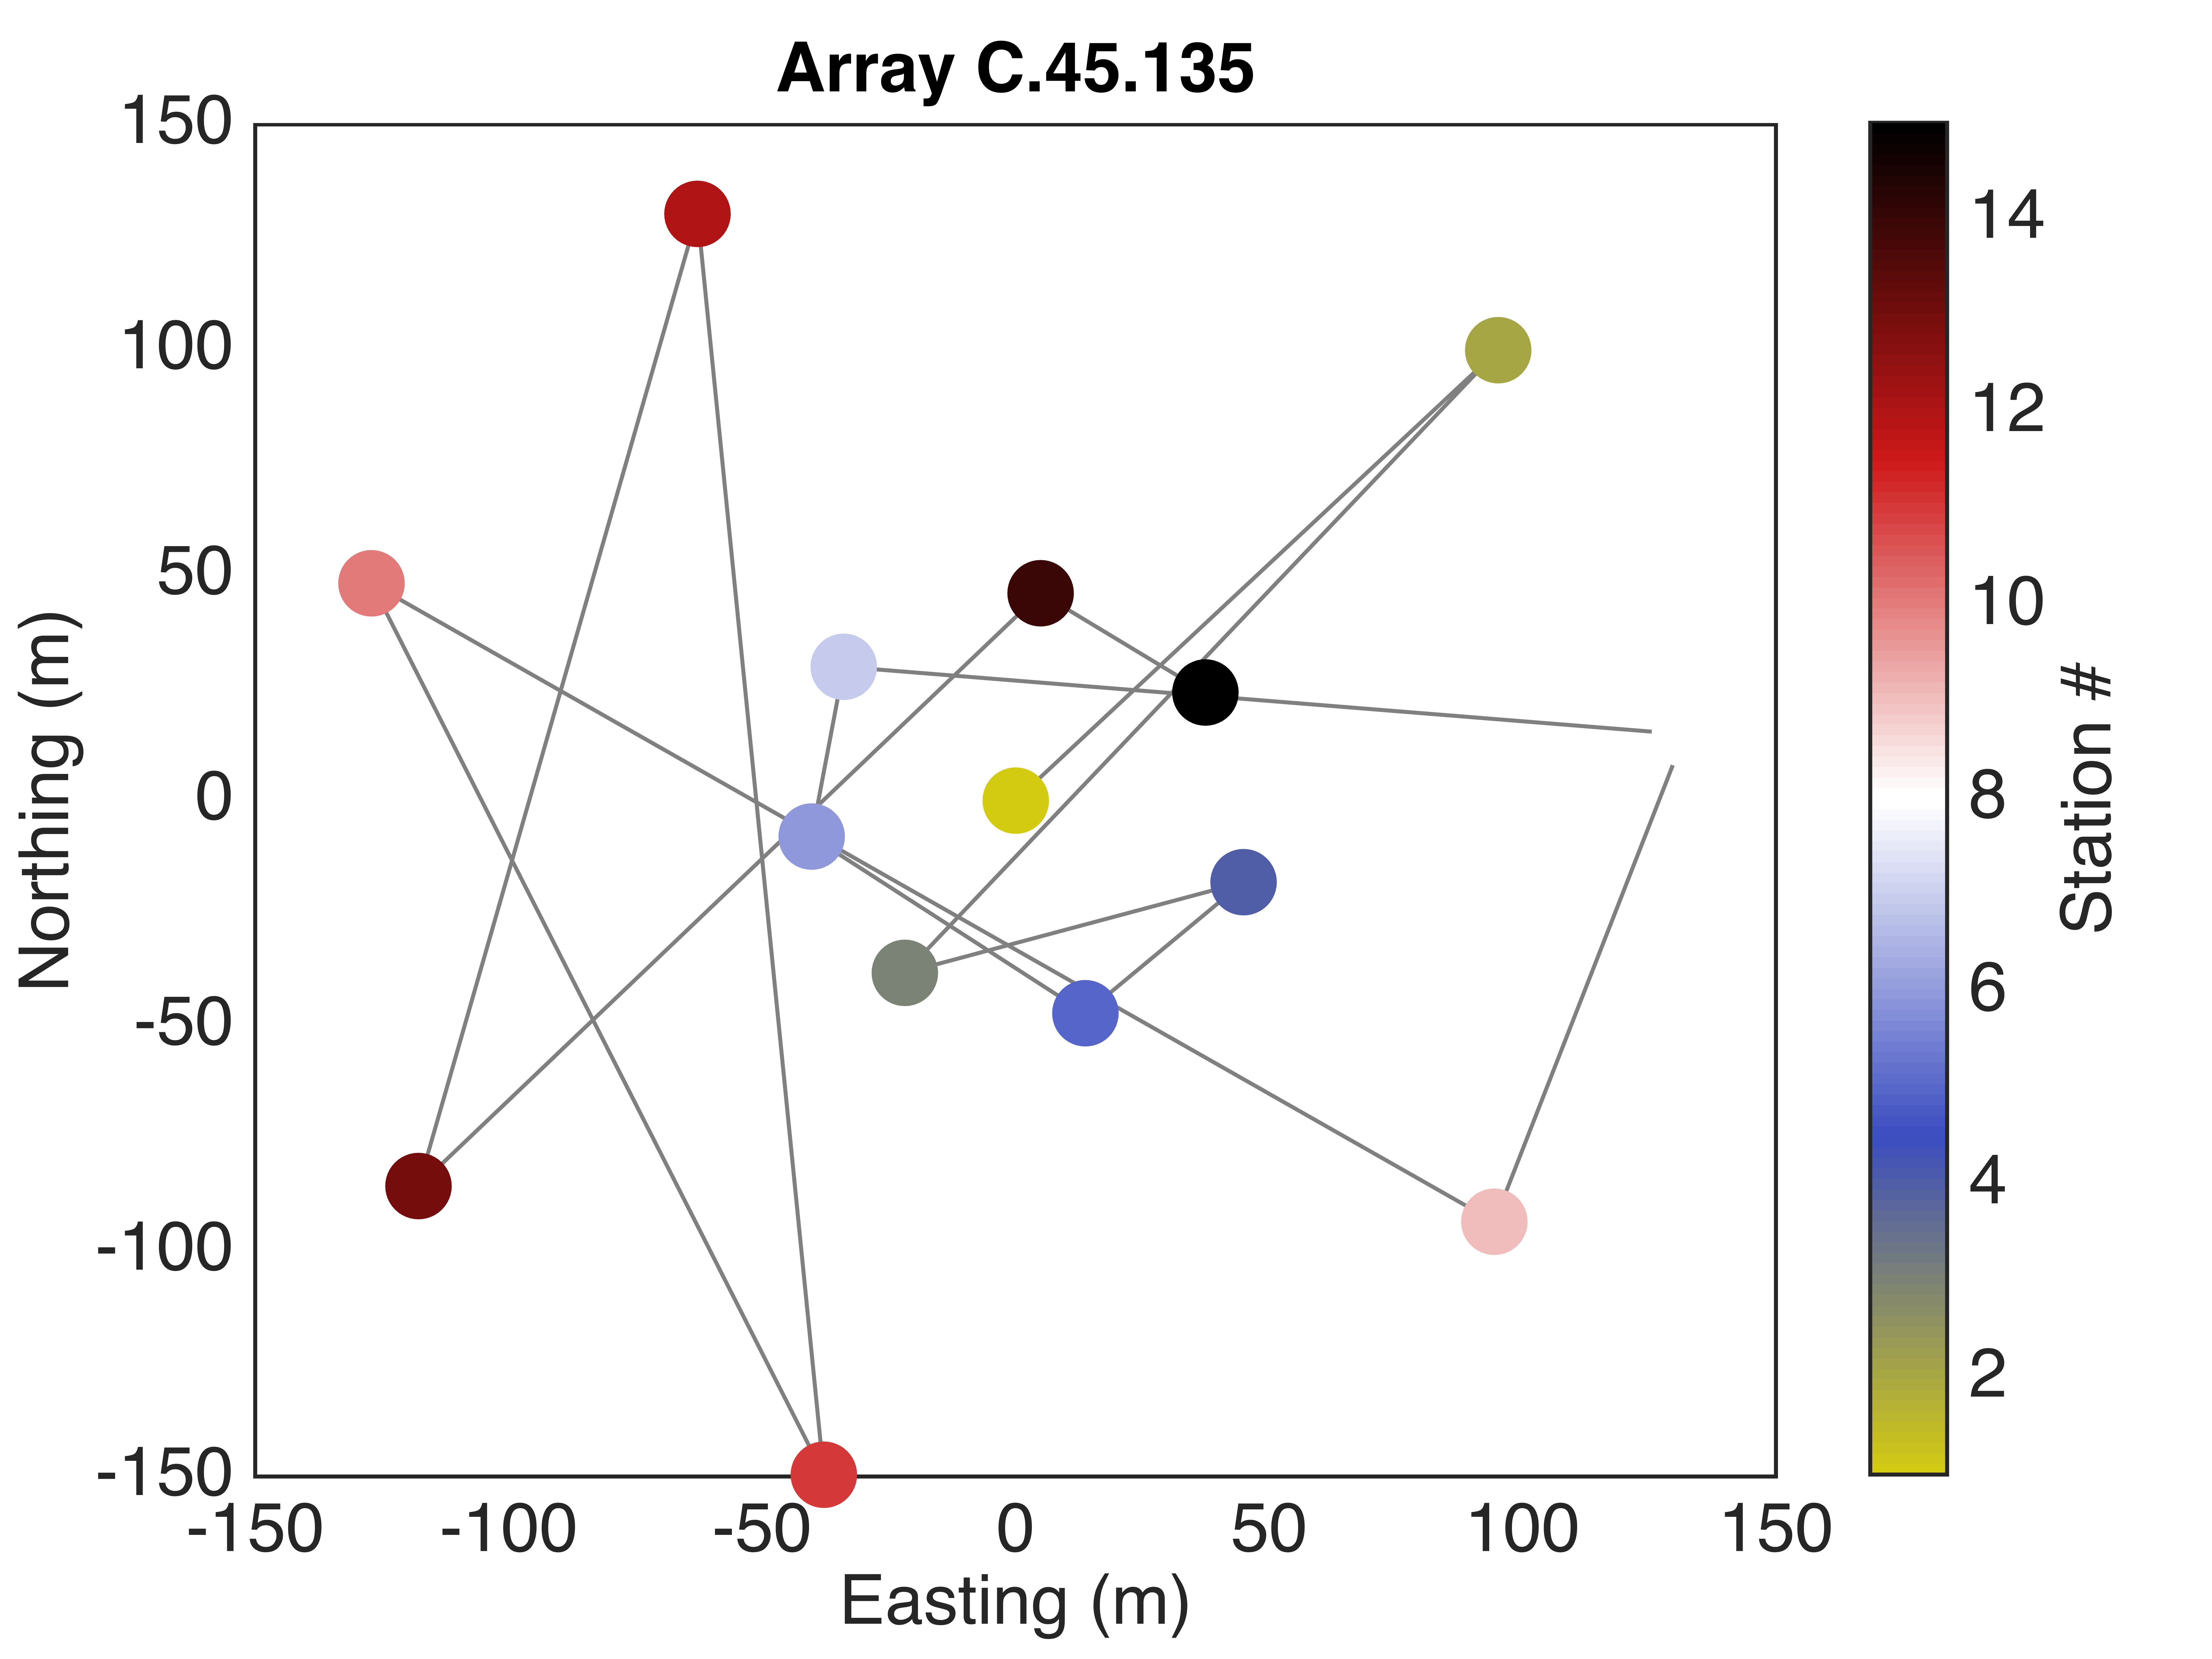
\includegraphics[width=\textwidth]{../pics/C-45-135/array.png}
}
%--------------------------------------------------------------------
%            arrays                                                                                   
%--------------------------------------------------------------------
\frame
{
\frametitle{{\bf Array ``large"}}
\centering
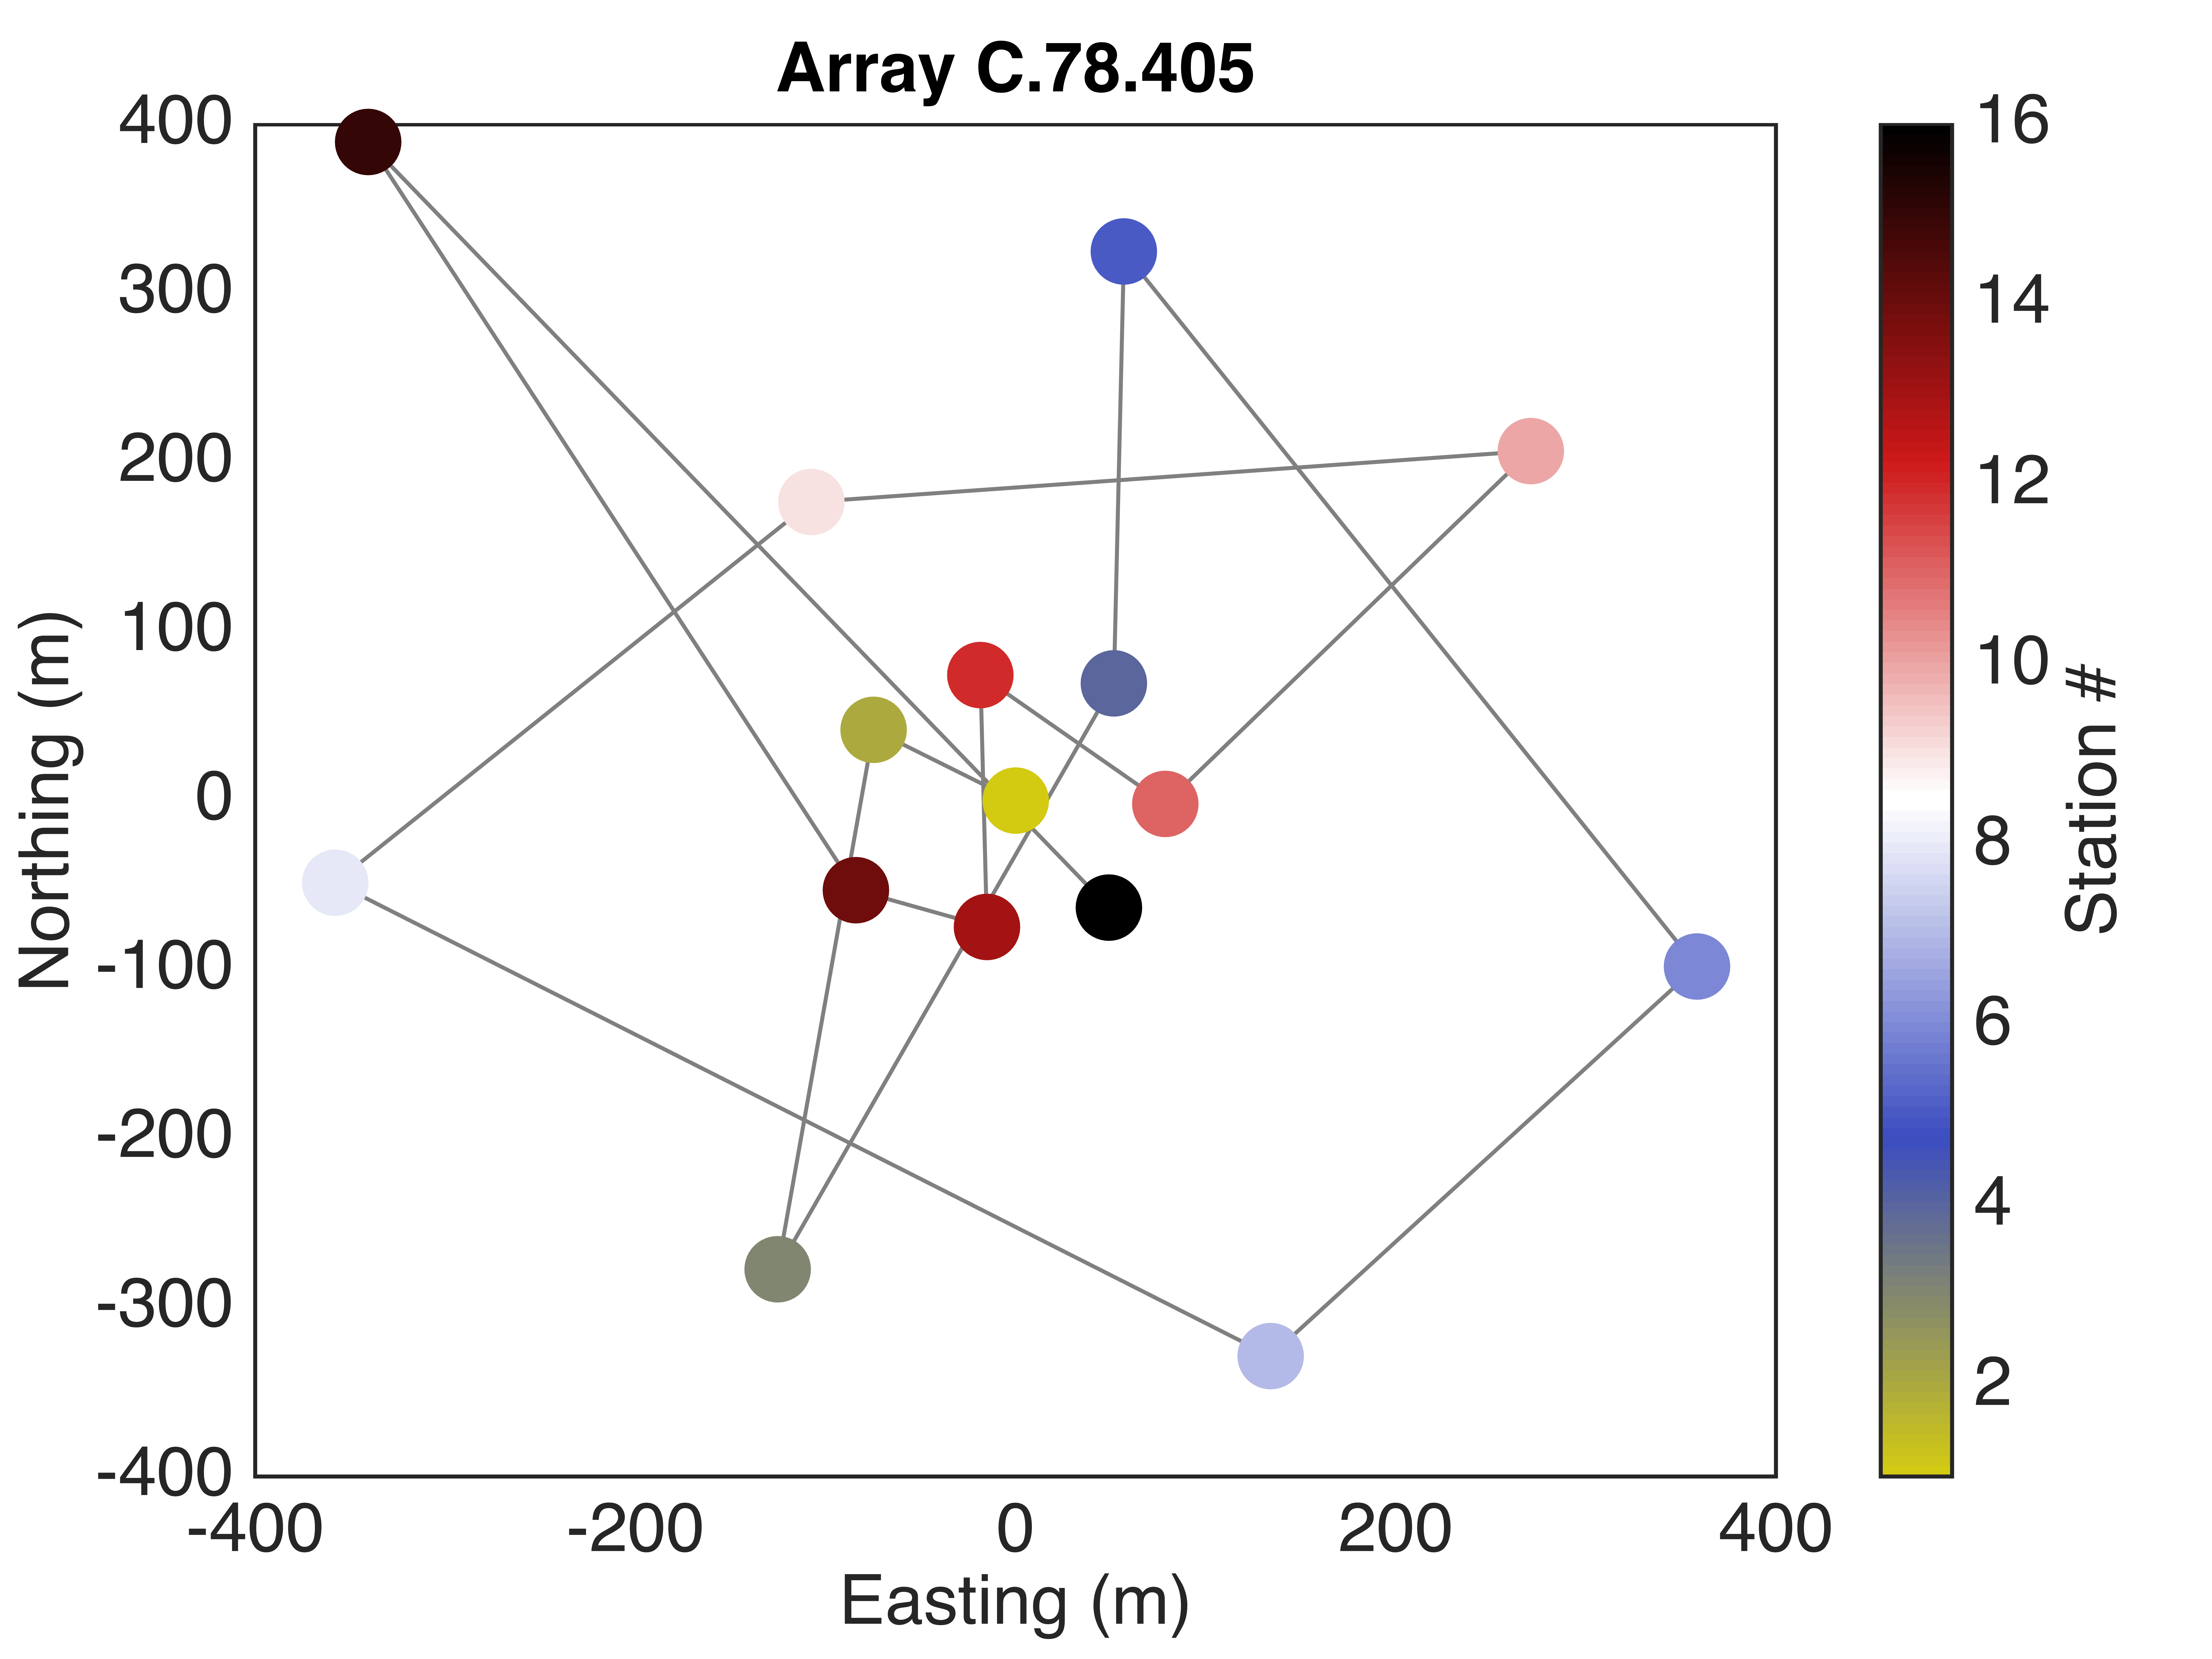
\includegraphics[width=\textwidth]{../pics/C-78-405/array.png}
}
%--------------------------------------------------------------------
%            arrays                                                                                   
%--------------------------------------------------------------------
\frame
{
\frametitle{{\bf All arrays}}
\centering
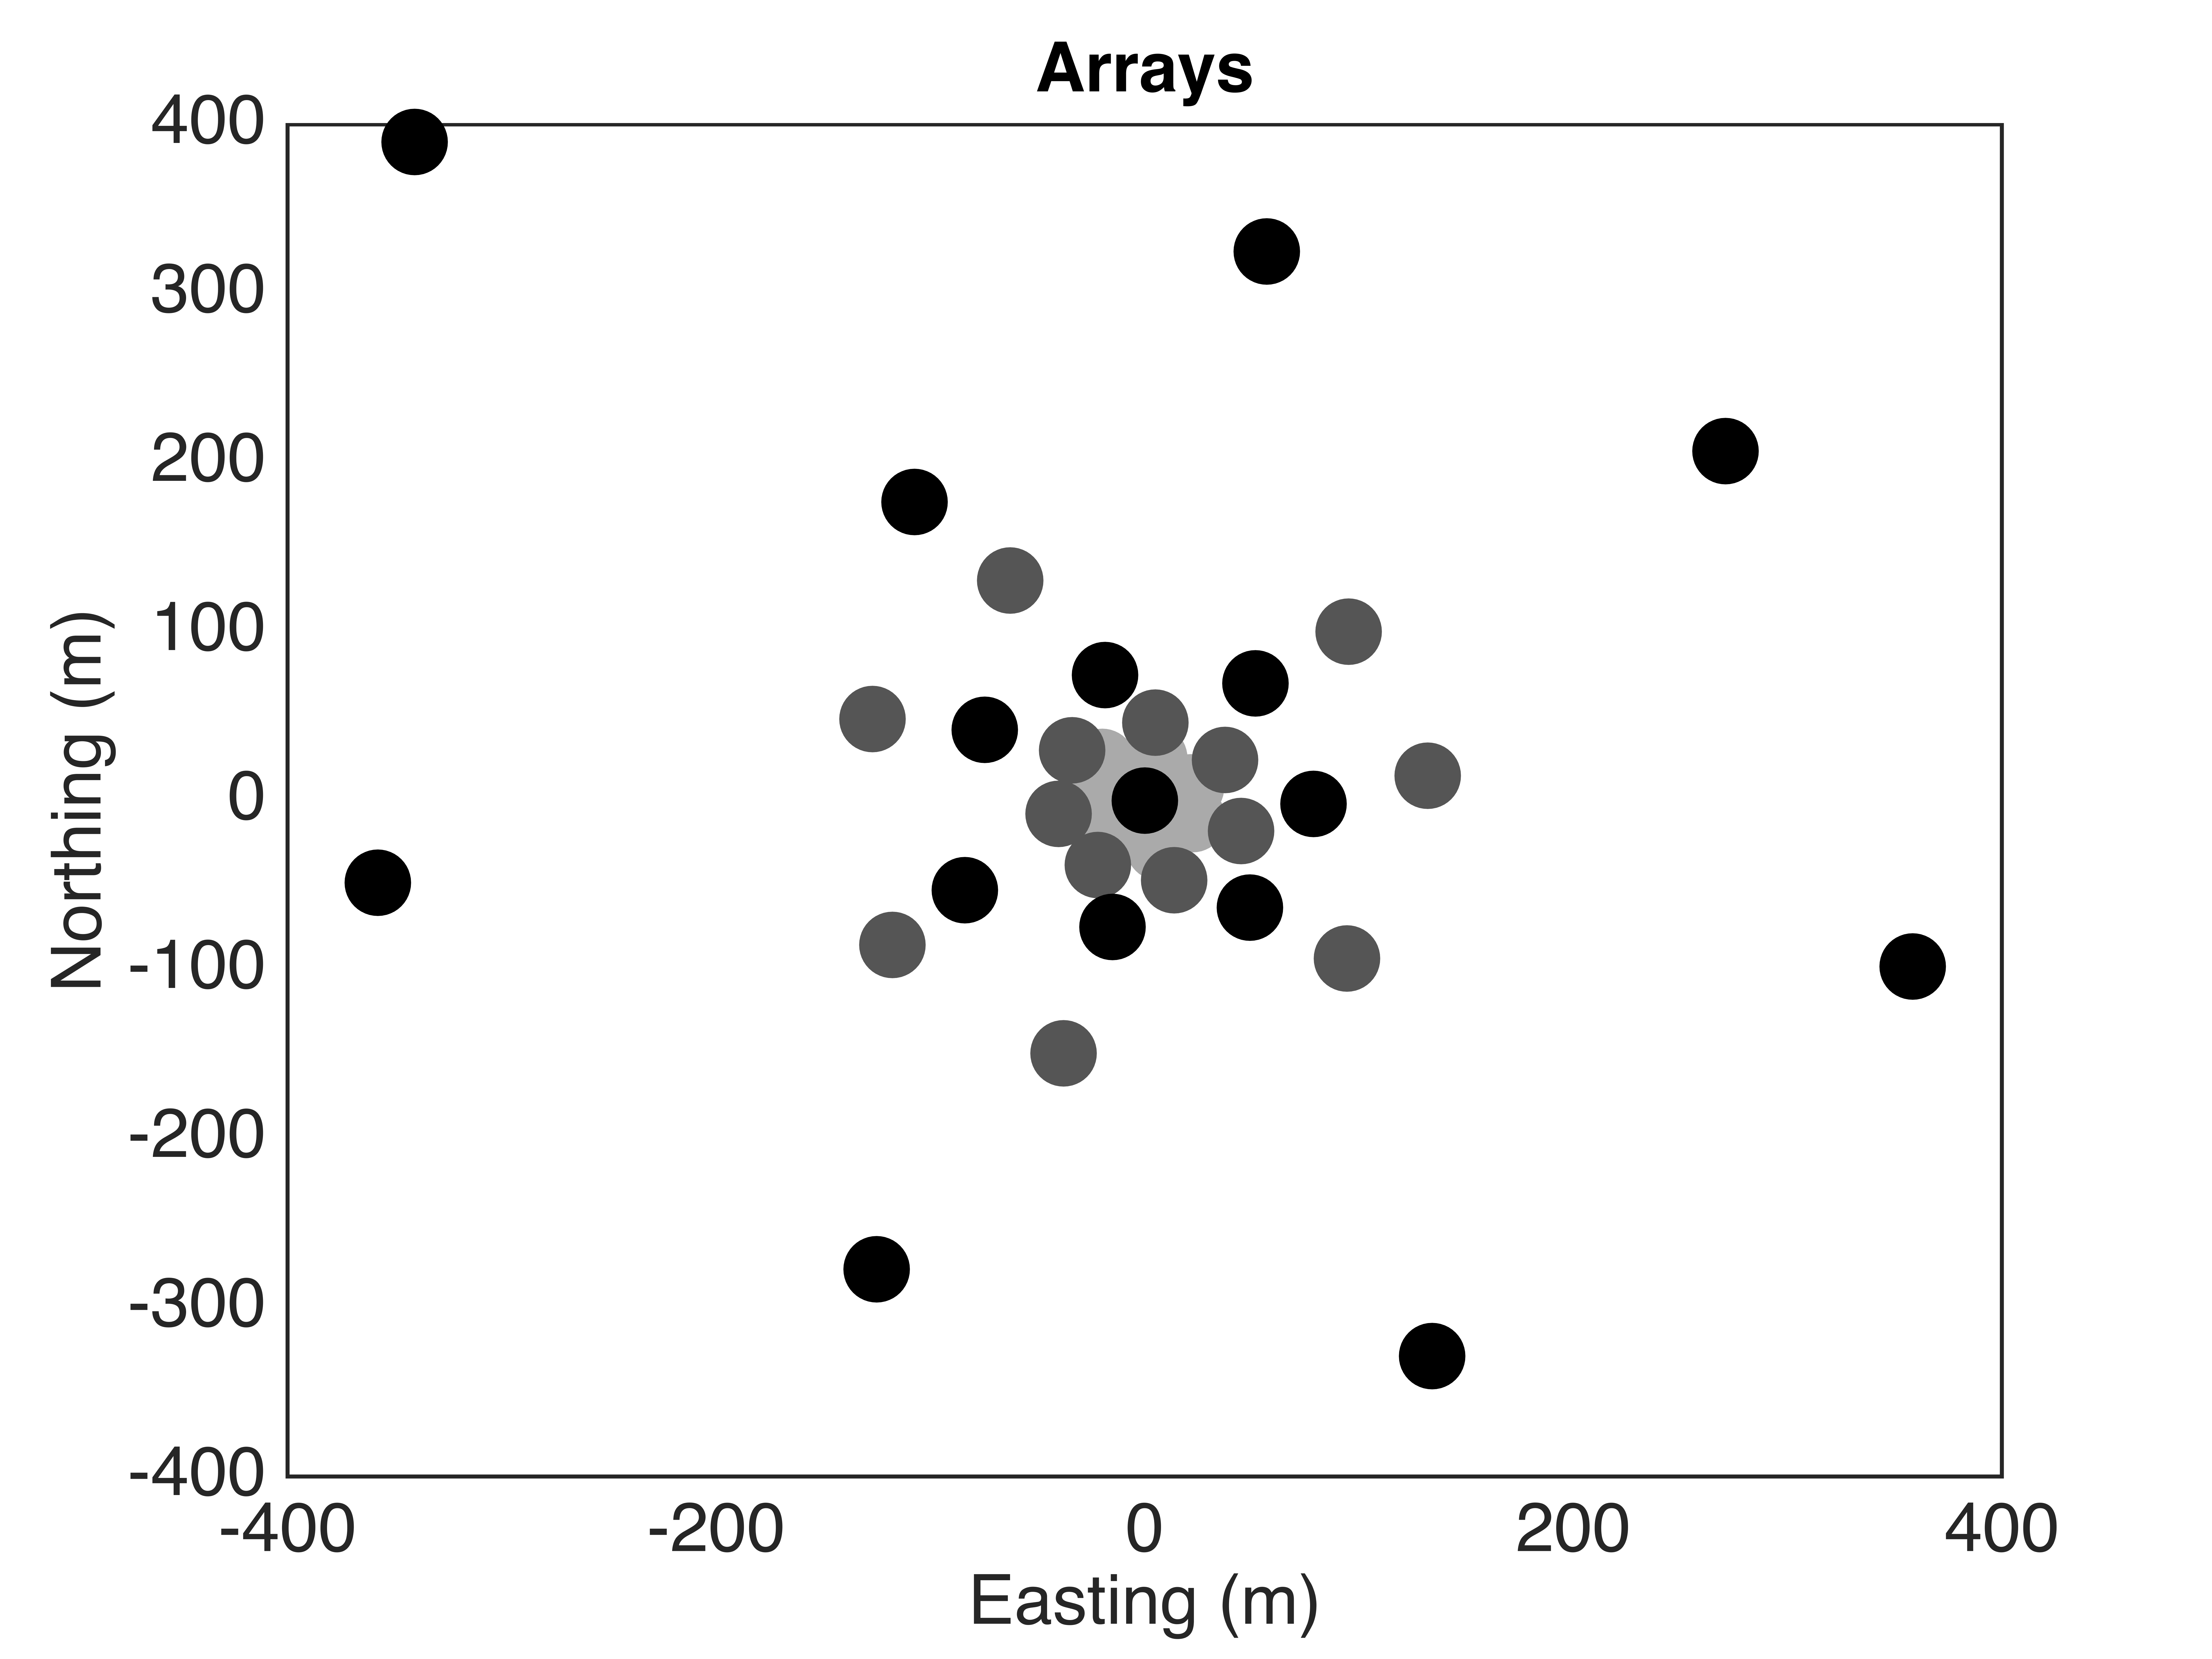
\includegraphics[width=0.9\textwidth]{../pics/arrays.png}
\vfill
it's a white walker signal (spiral)
}
%--------------------------------------------------------------------
%            arrays                                                                                   
%--------------------------------------------------------------------
\frame
{
\frametitle{{\bf Arrays line}}
\centering
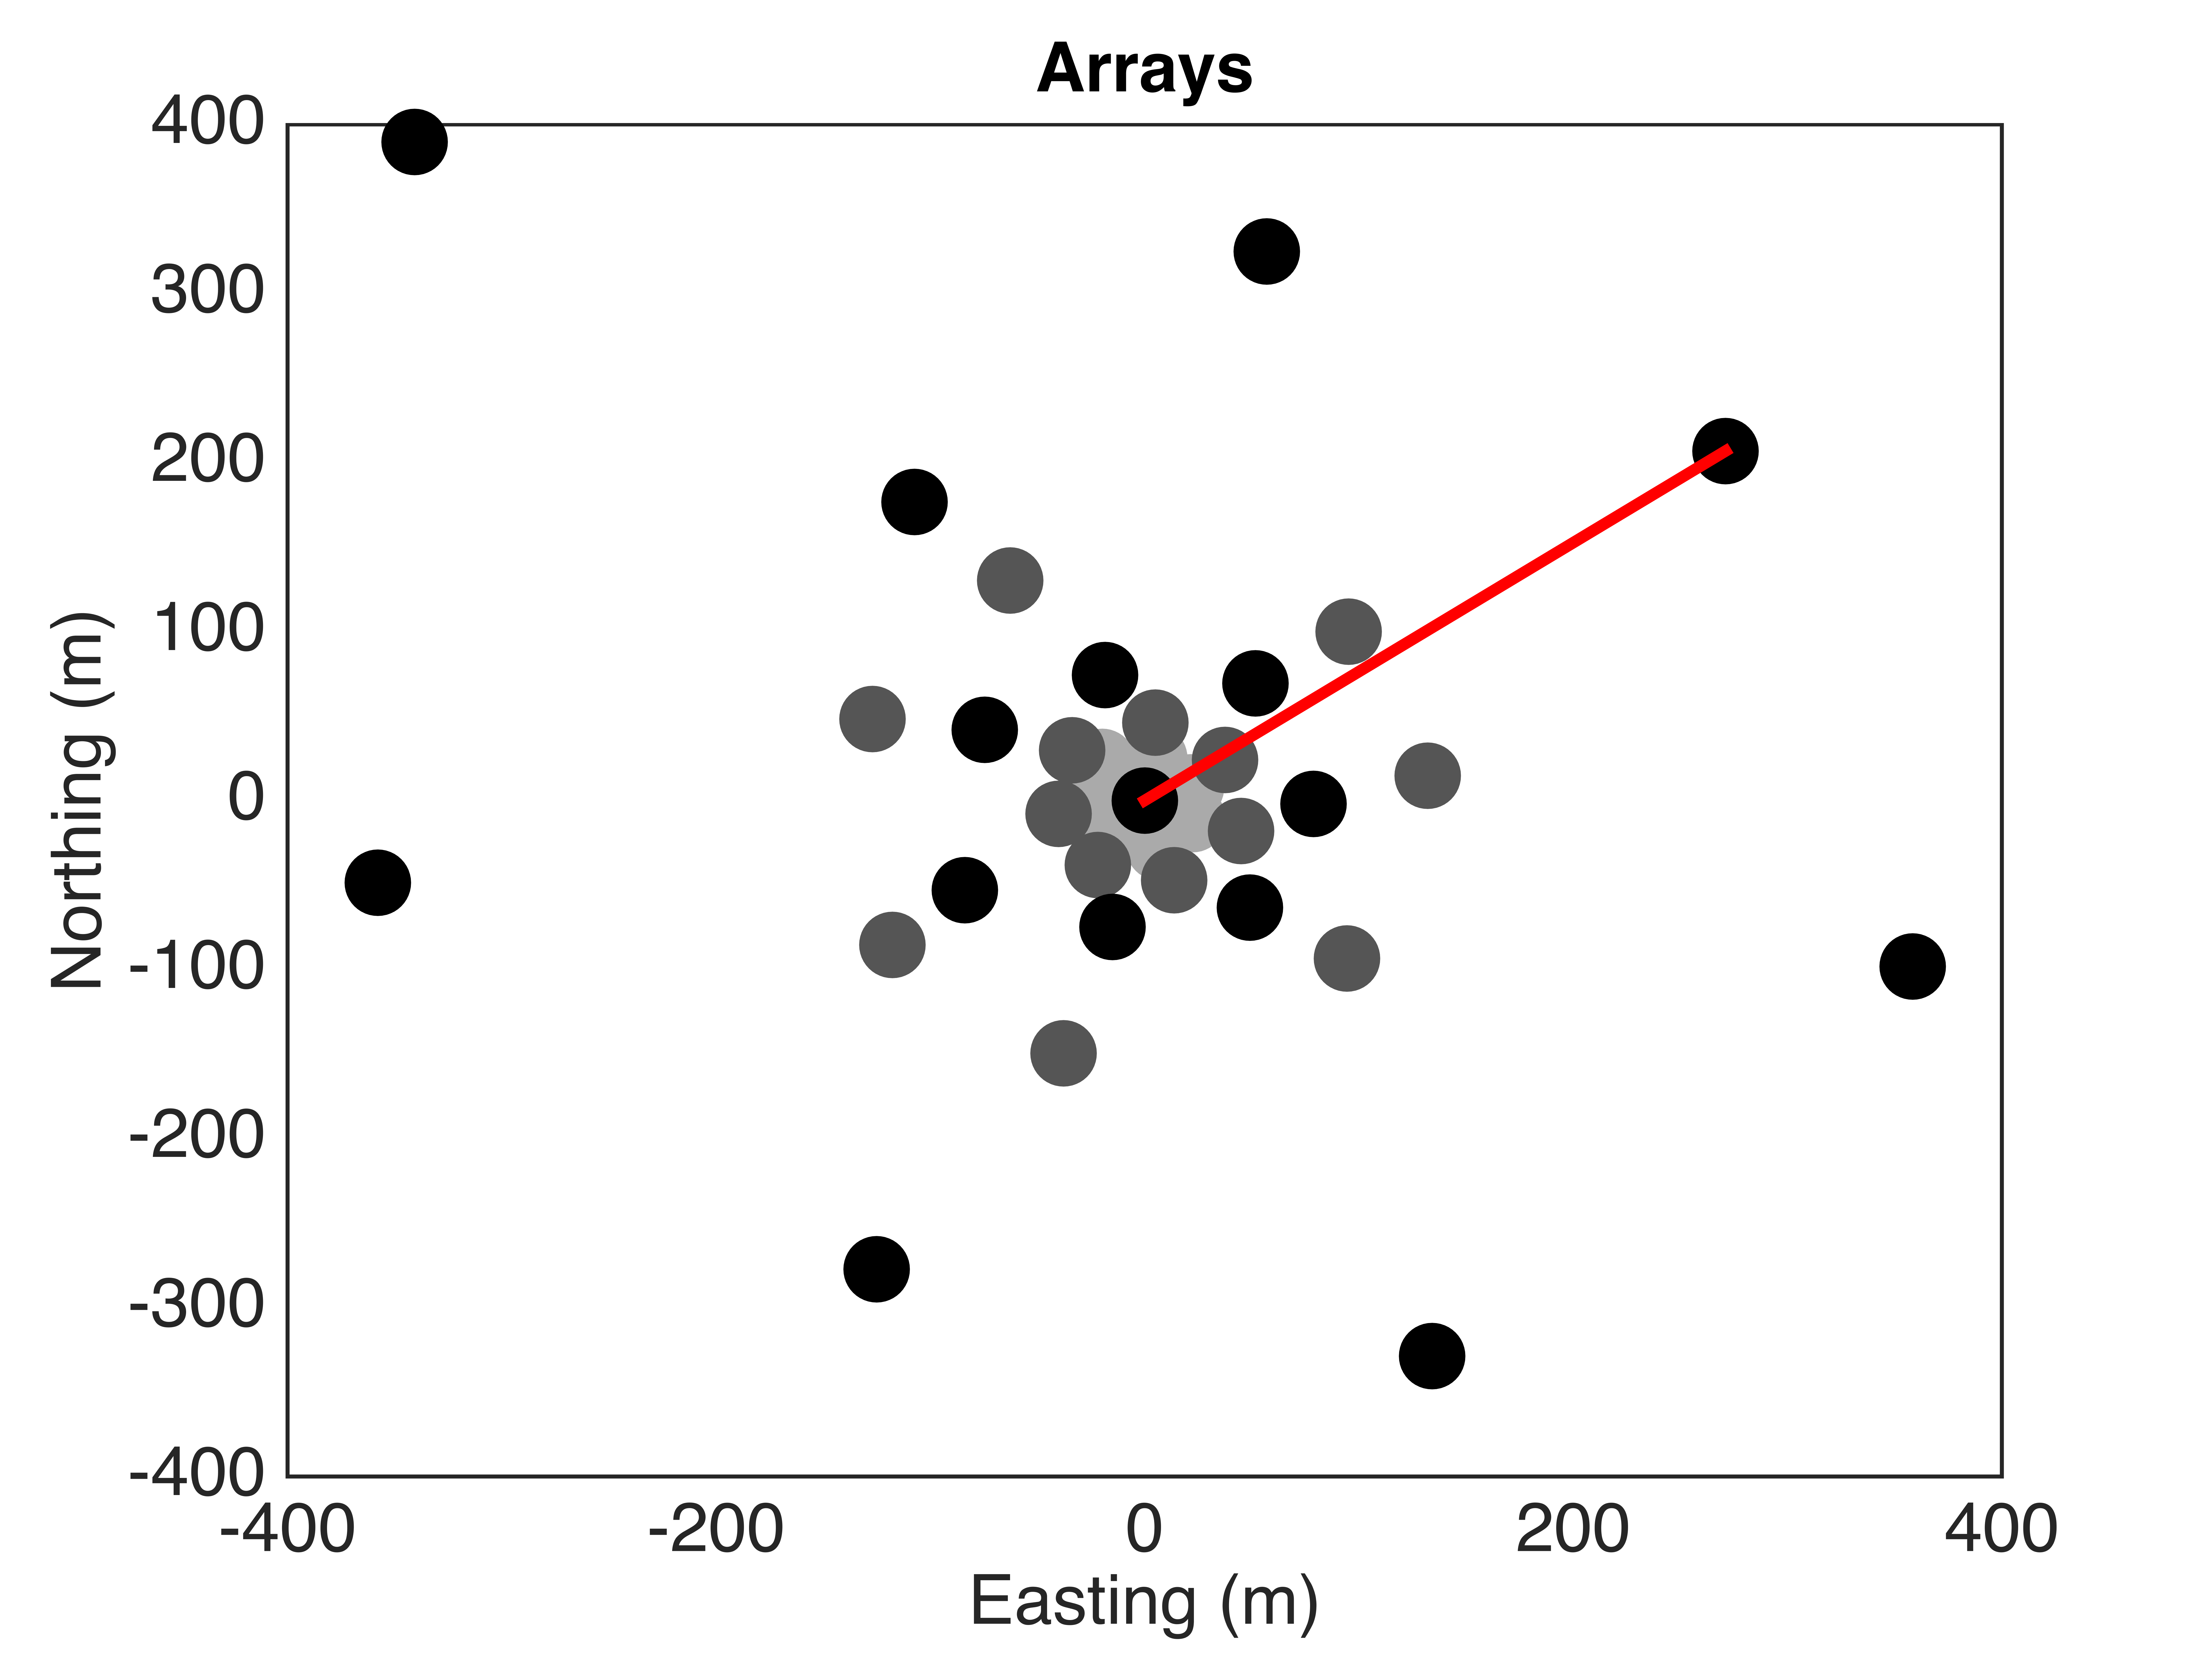
\includegraphics[width=0.9\textwidth]{../pics/arrays-line.png}
\vfill
stations 8, 15 and 10 of arrays small, medium and large respectively
}
%--------------------------------------------------------------------
%            noise                                                                                  
%--------------------------------------------------------------------
\frame
{
\frametitle{{\bf Noise sources}}
\centering
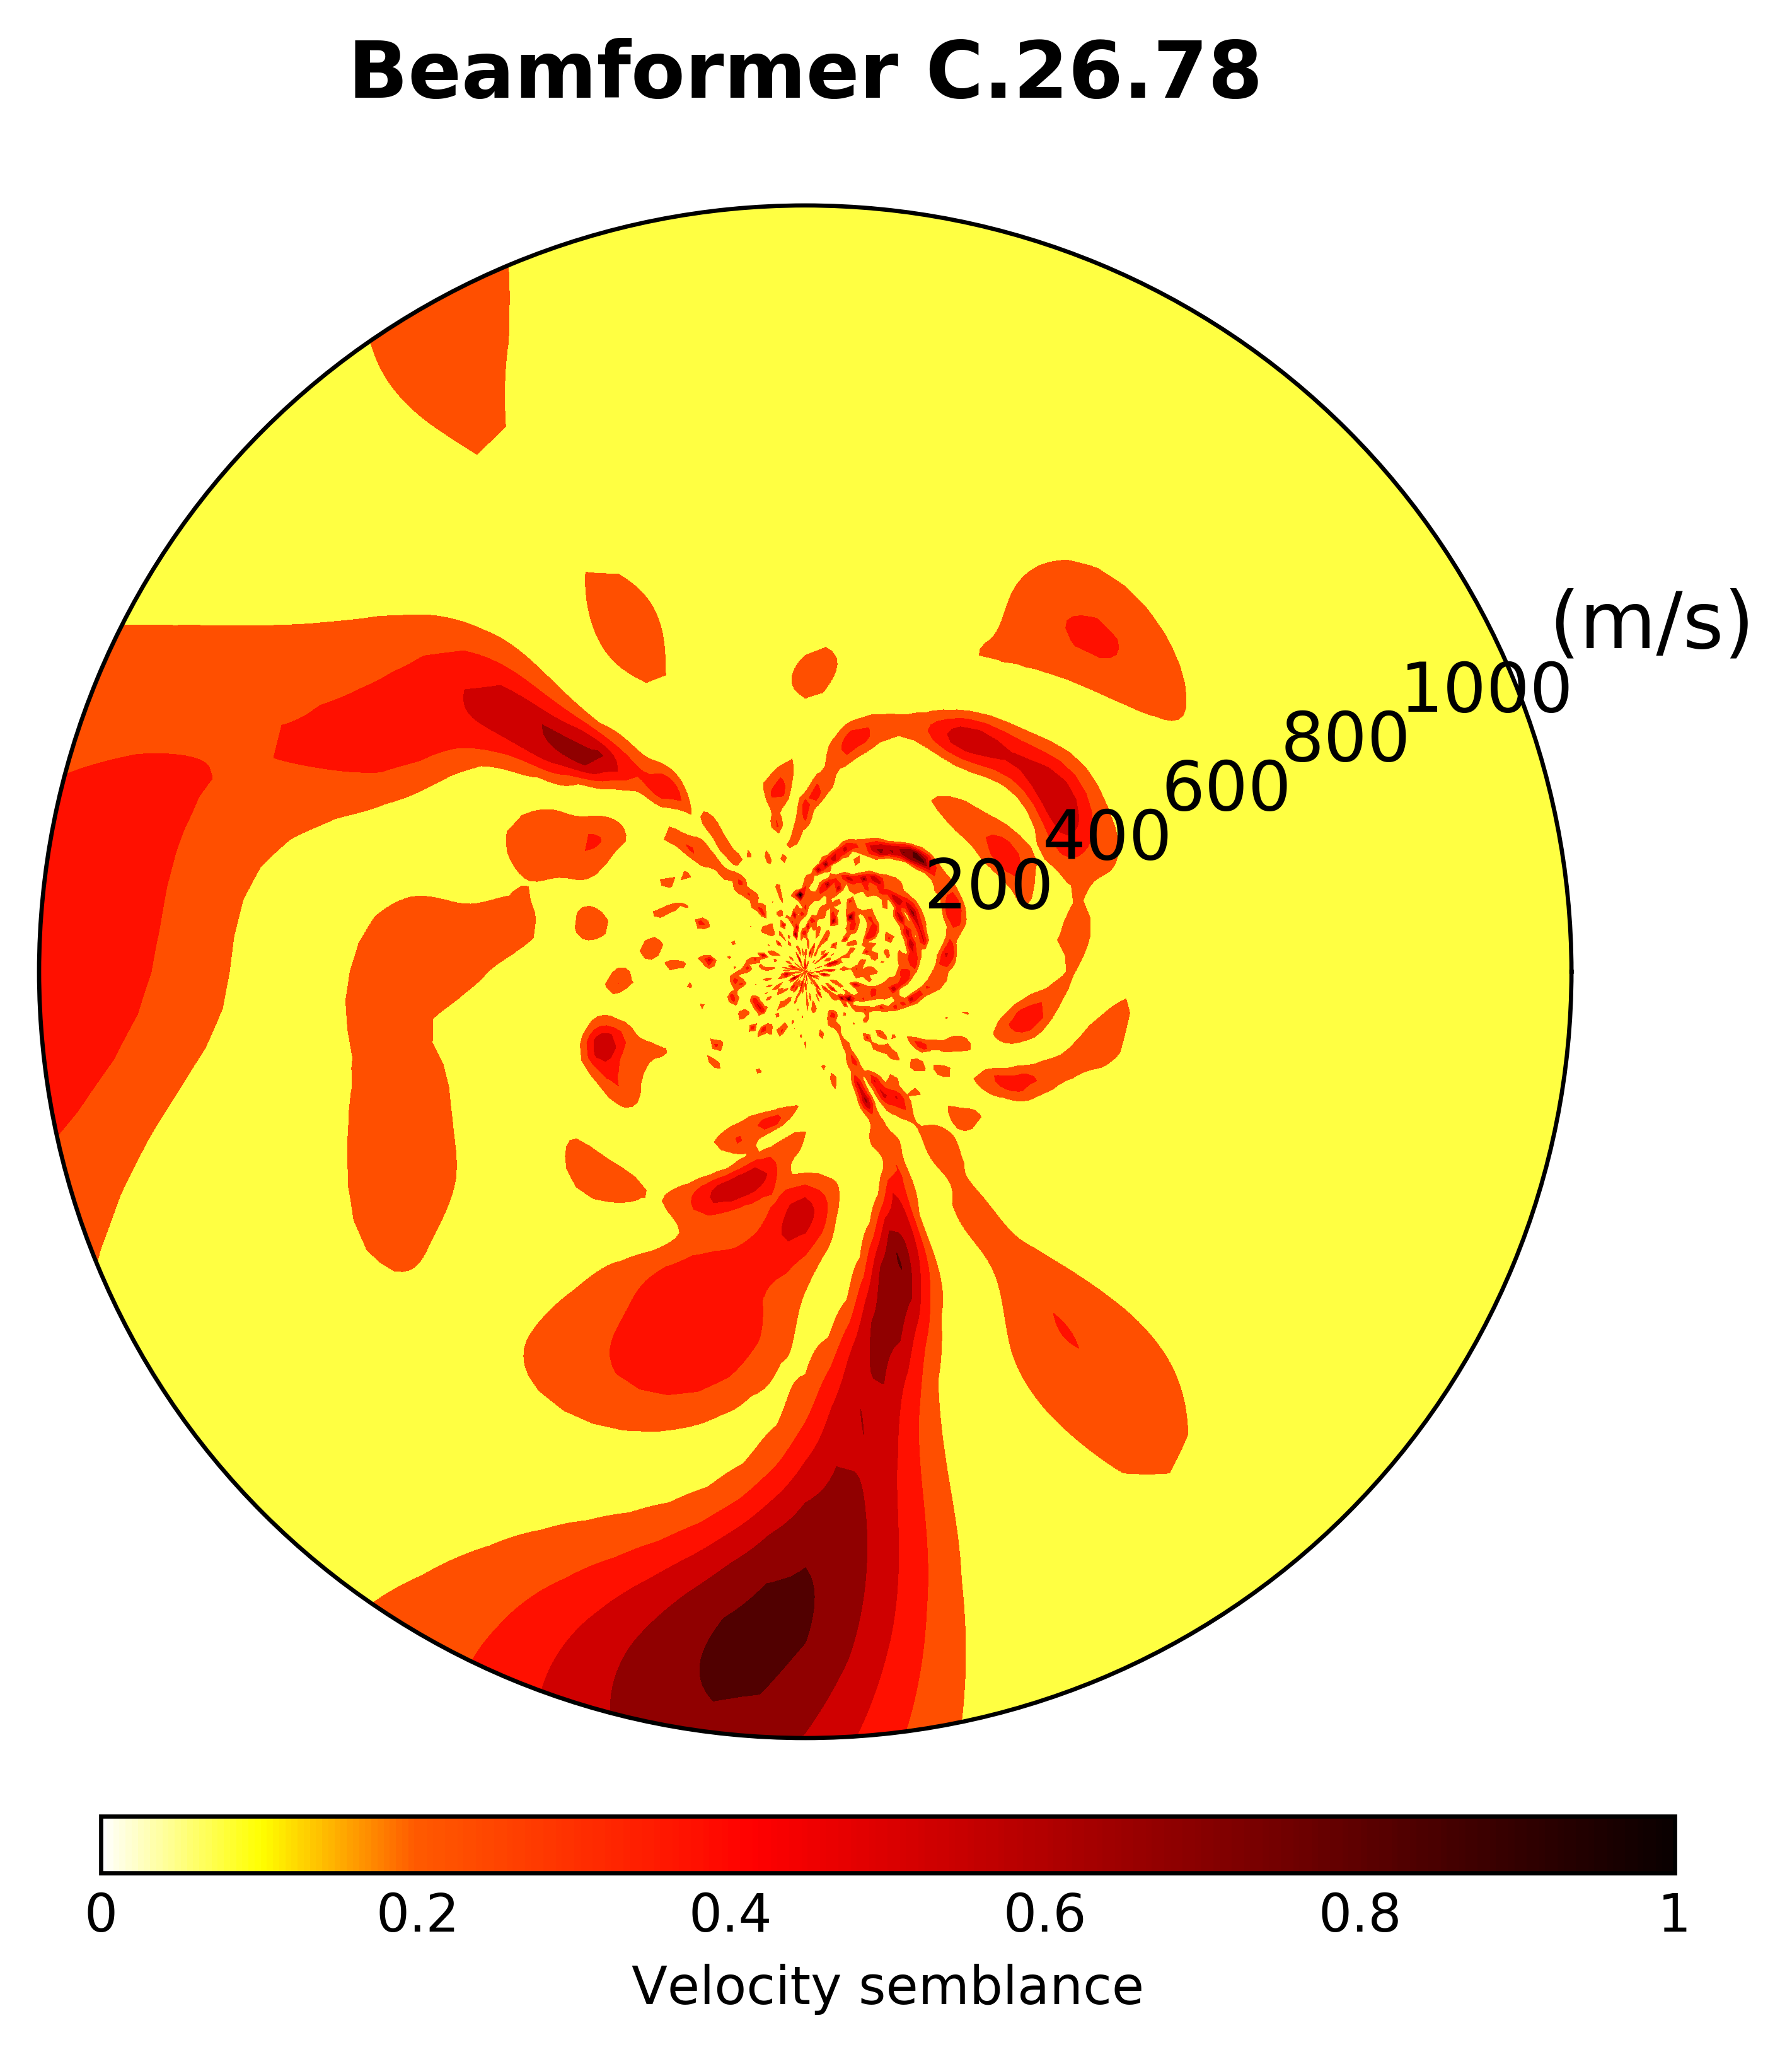
\includegraphics[width=0.65\textwidth]{../pics/C-26-78/beamformer.png}
}
%--------------------------------------------------------------------
%            noise                                                                                  
%--------------------------------------------------------------------
\frame
{
\frametitle{{\bf Noise sources}}
\centering
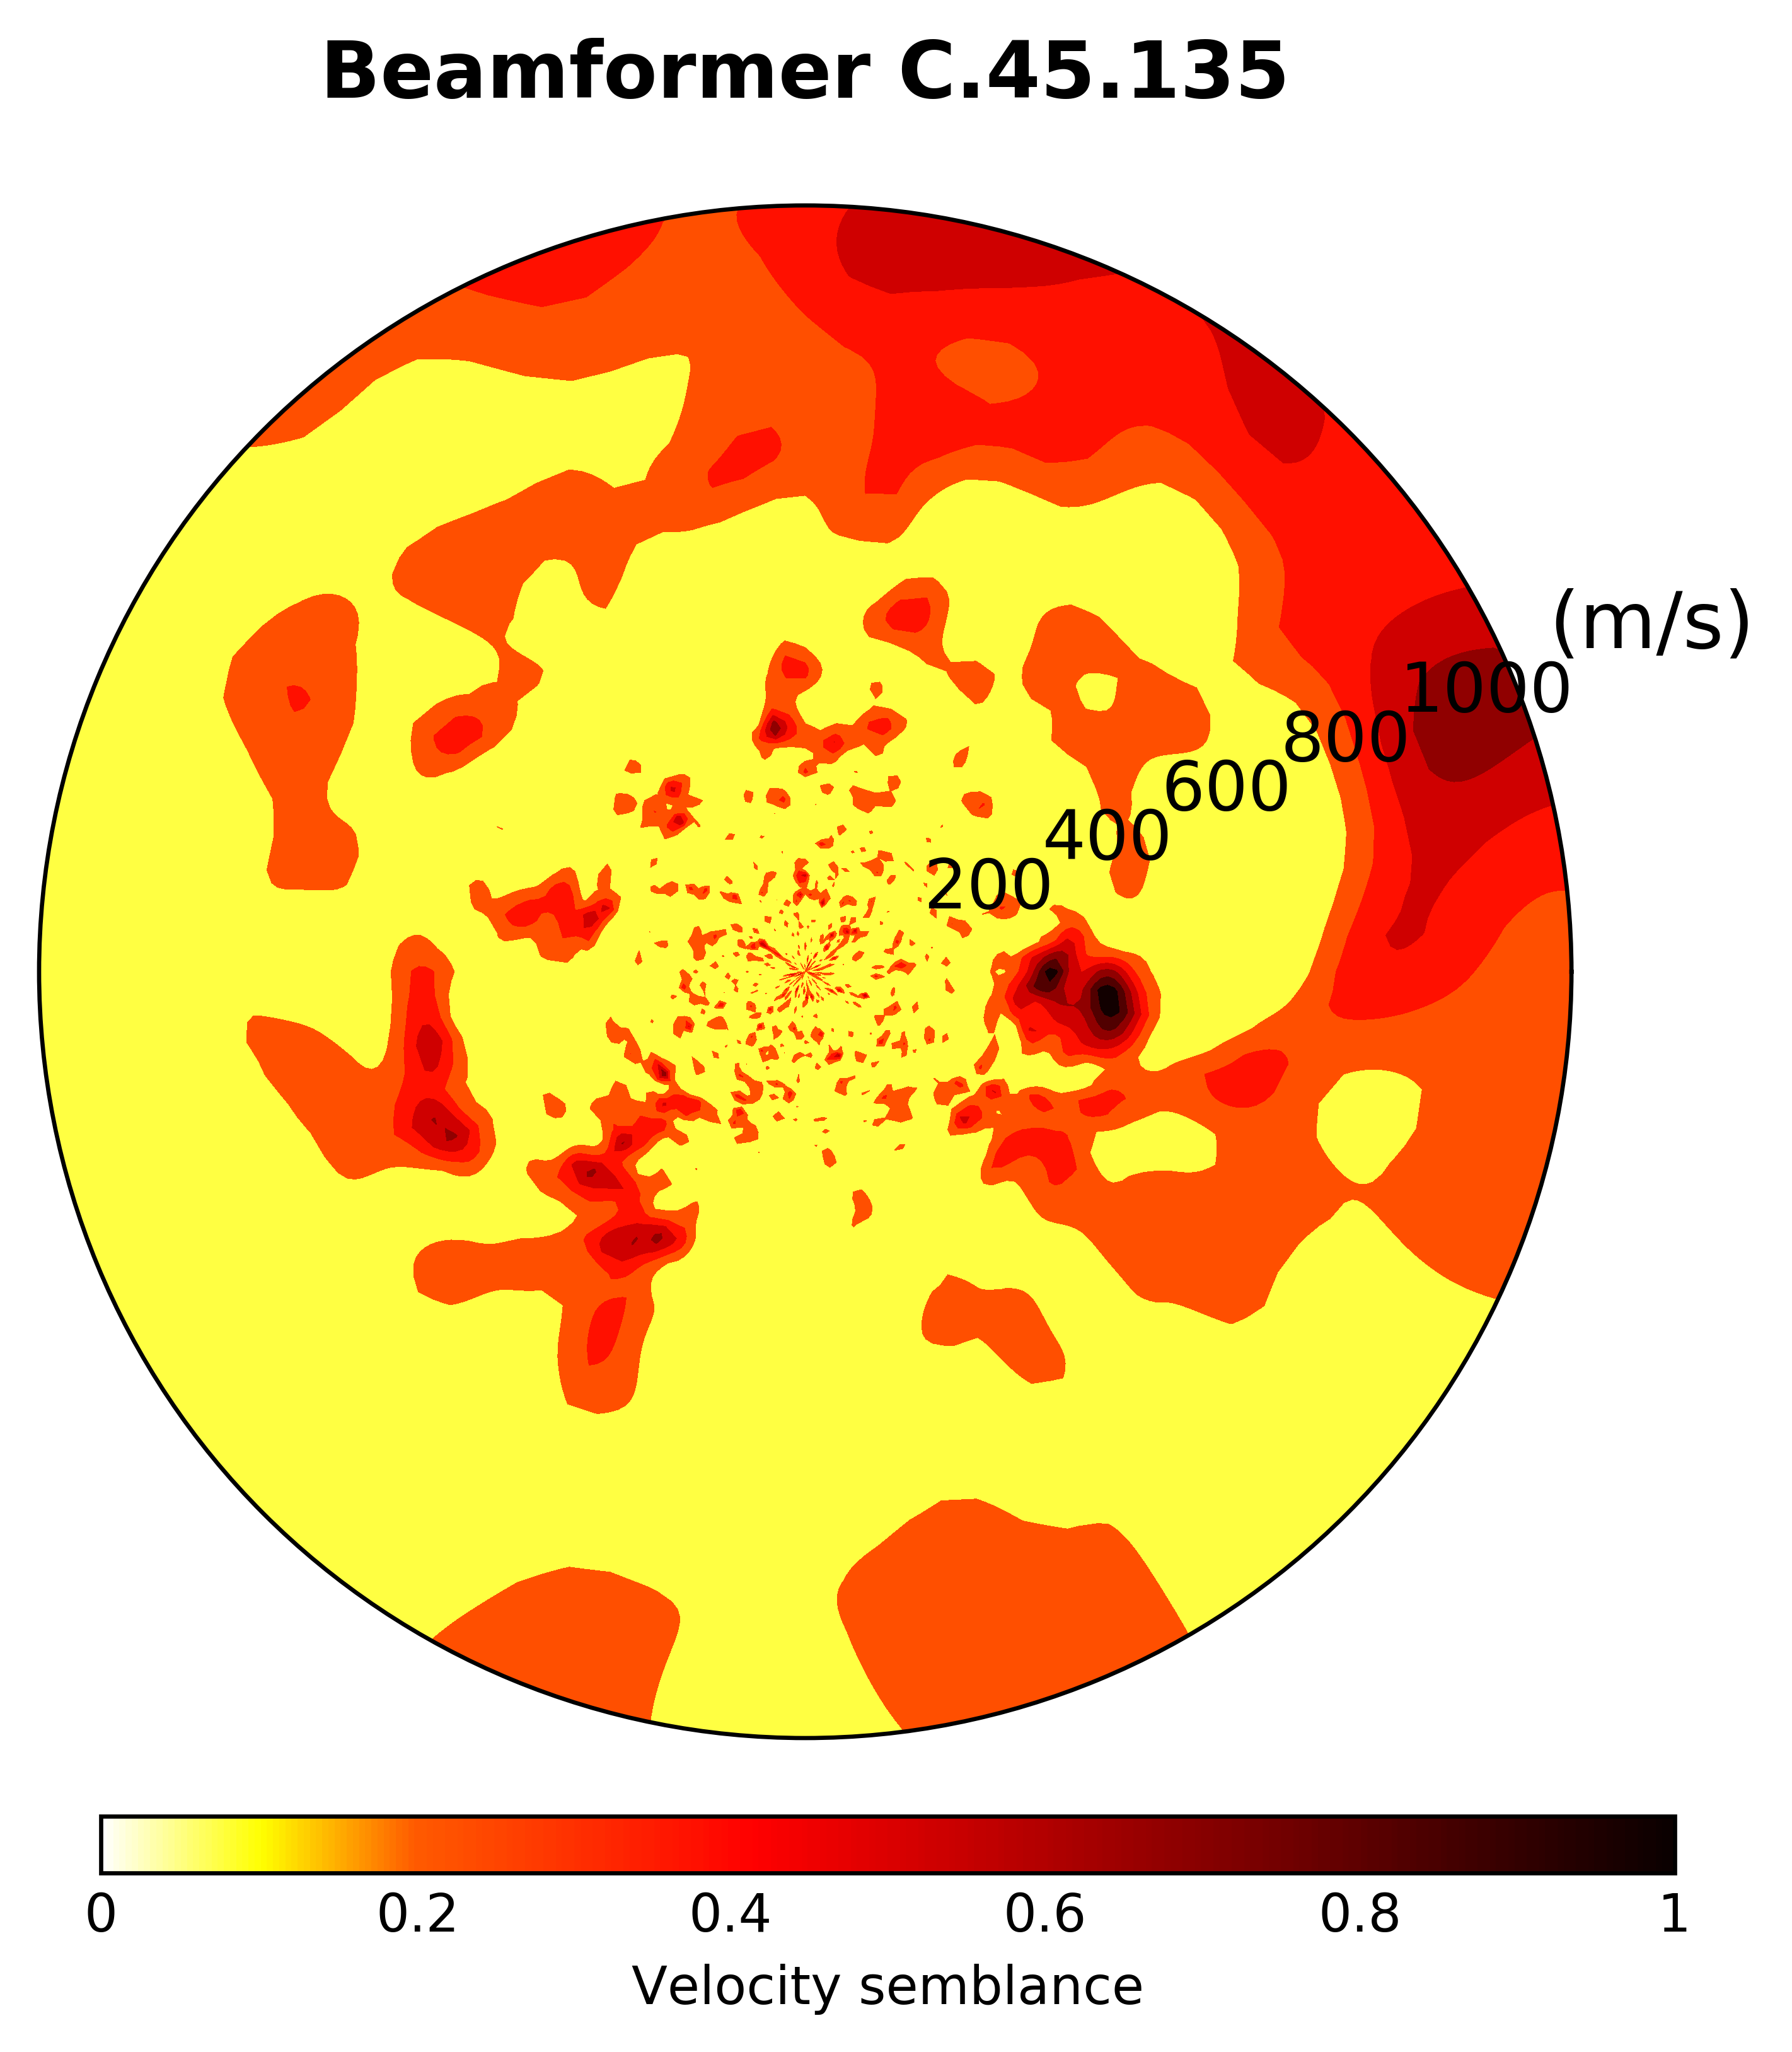
\includegraphics[width=0.65\textwidth]{../pics/C-45-135/beamformer.png}
}
%--------------------------------------------------------------------
%            noise                                                                                  
%--------------------------------------------------------------------
\frame
{
\frametitle{{\bf Noise sources}}
\centering
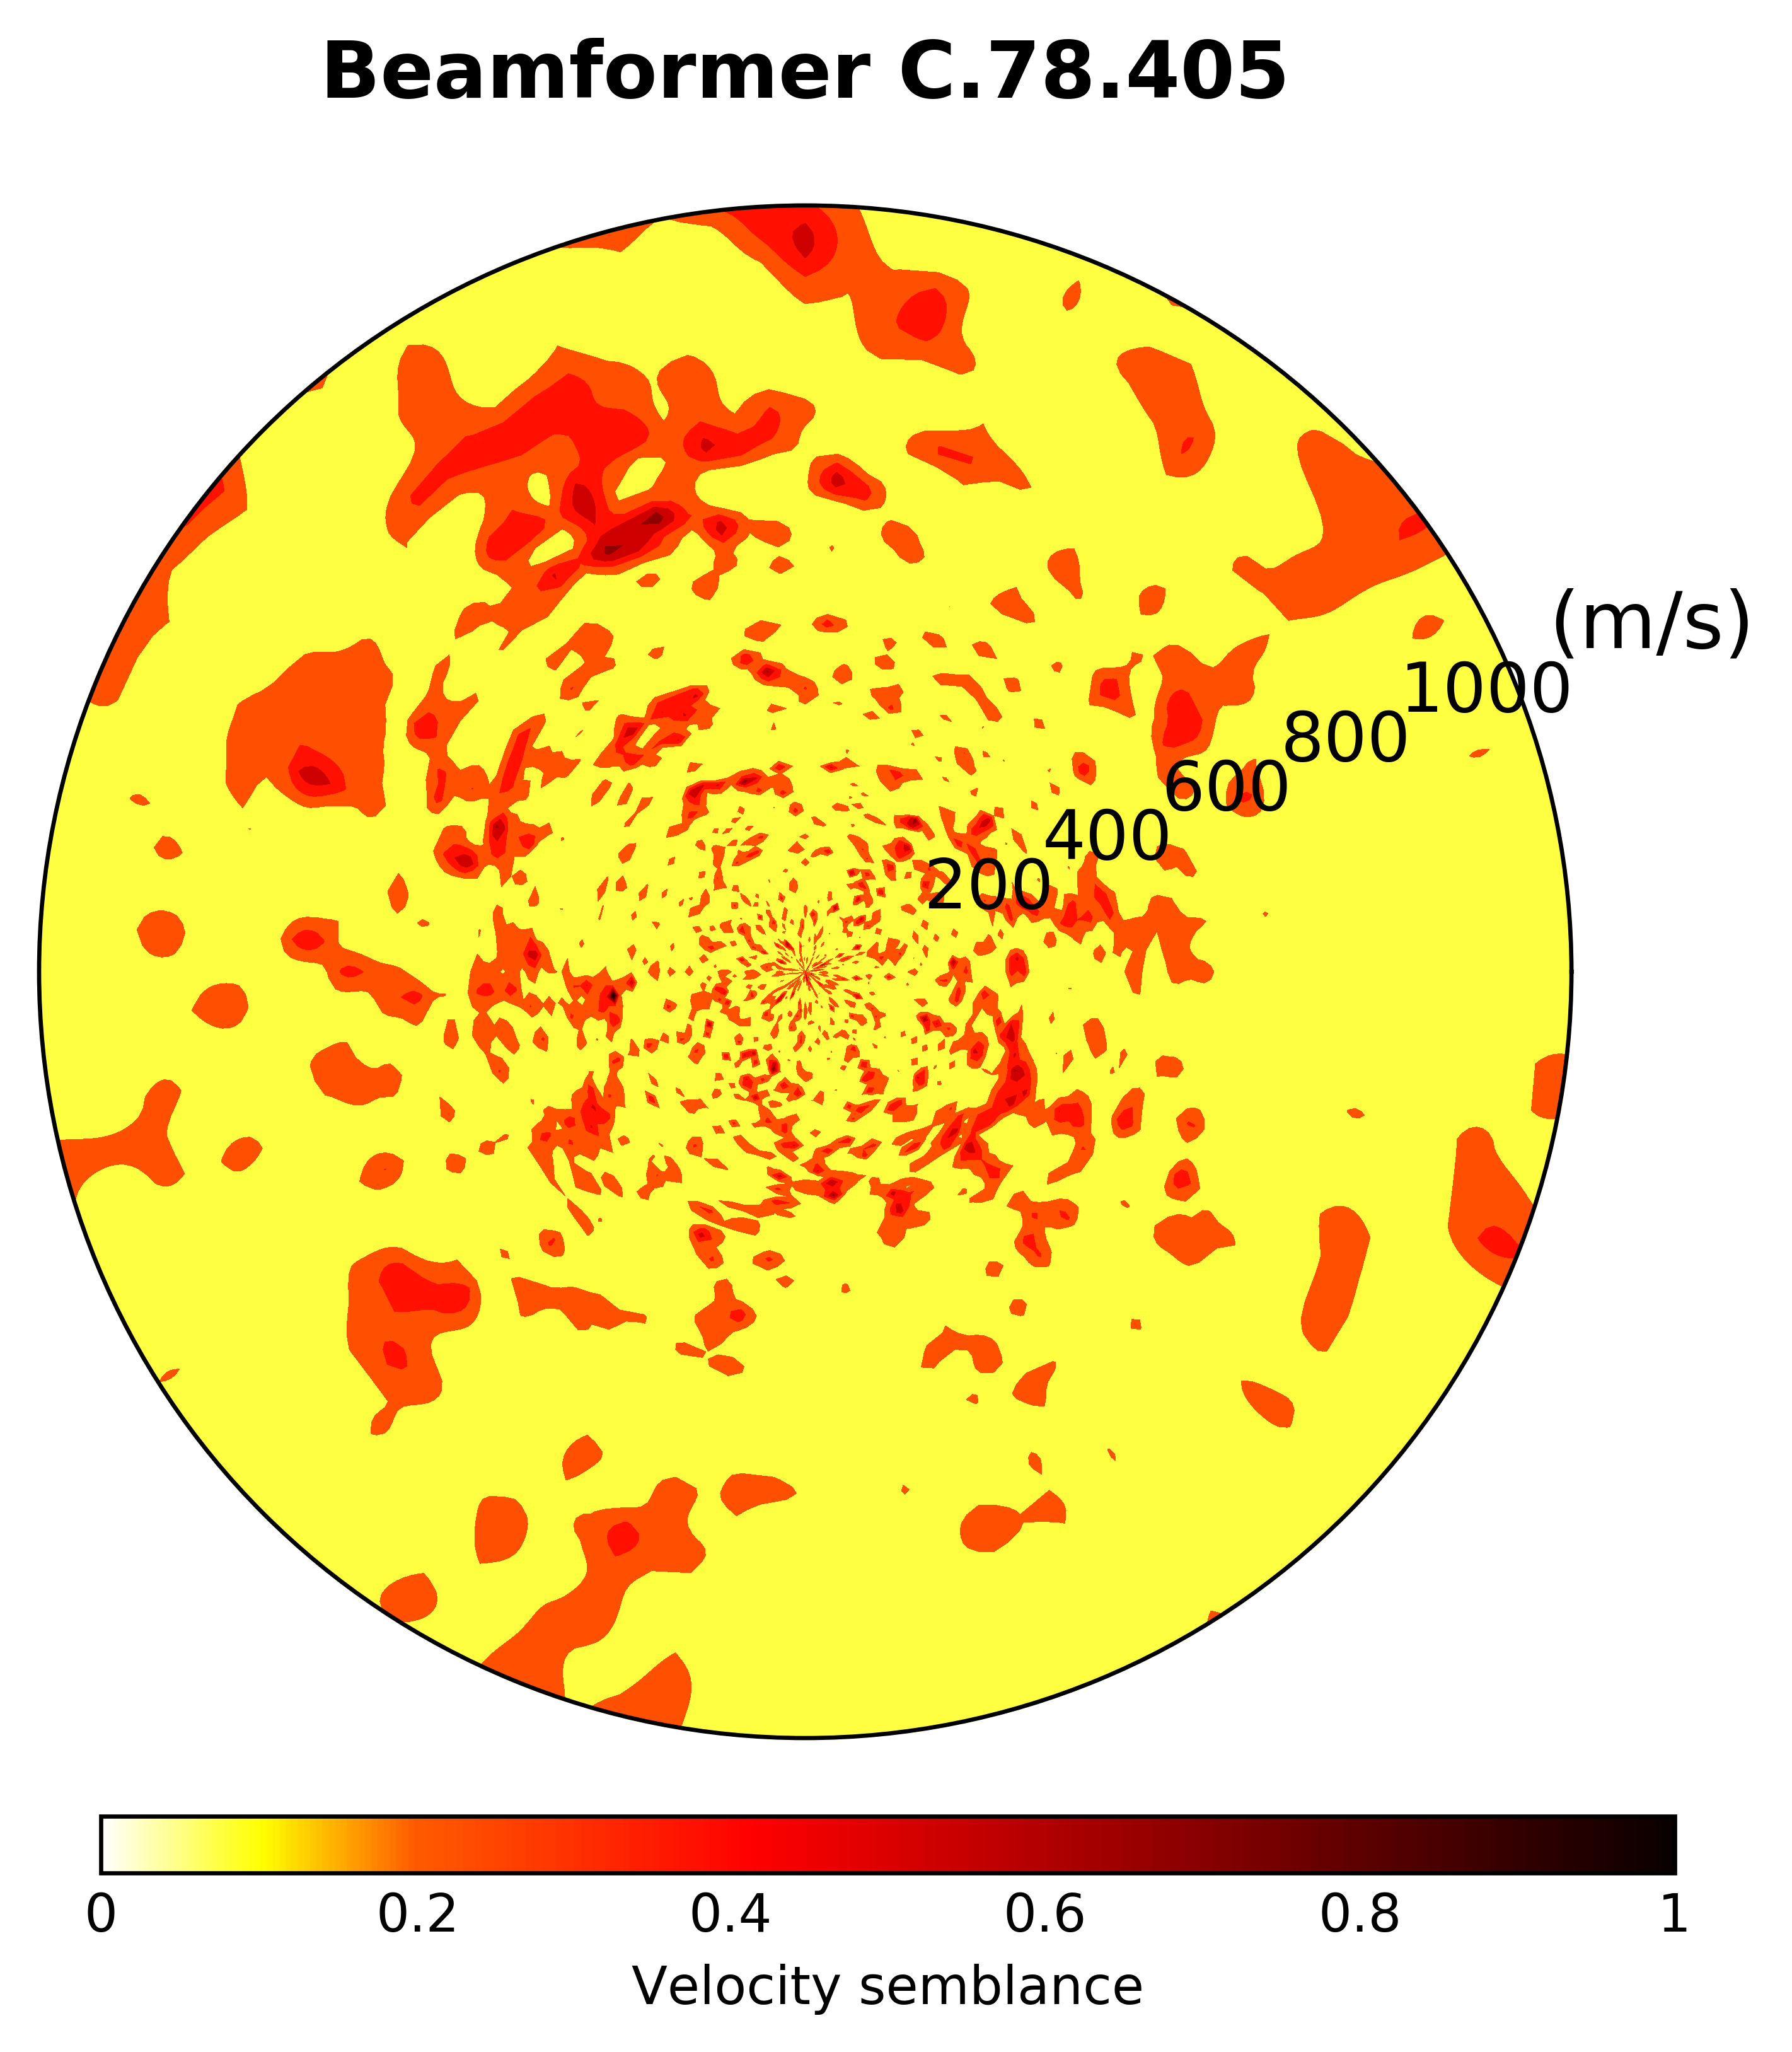
\includegraphics[width=0.65\textwidth]{../pics/C-78-405/beamformer.png}
}
%--------------------------------------------------------------------
%            data                                                                                   
%--------------------------------------------------------------------
\frame
{
\centering
{\bf On y vamos!}
}
%--------------------------------------------------------------------
%            group velocity                                                                                   
%--------------------------------------------------------------------
\frame
{
\frametitle{{\bf Group velocity ``small"}}
\centering
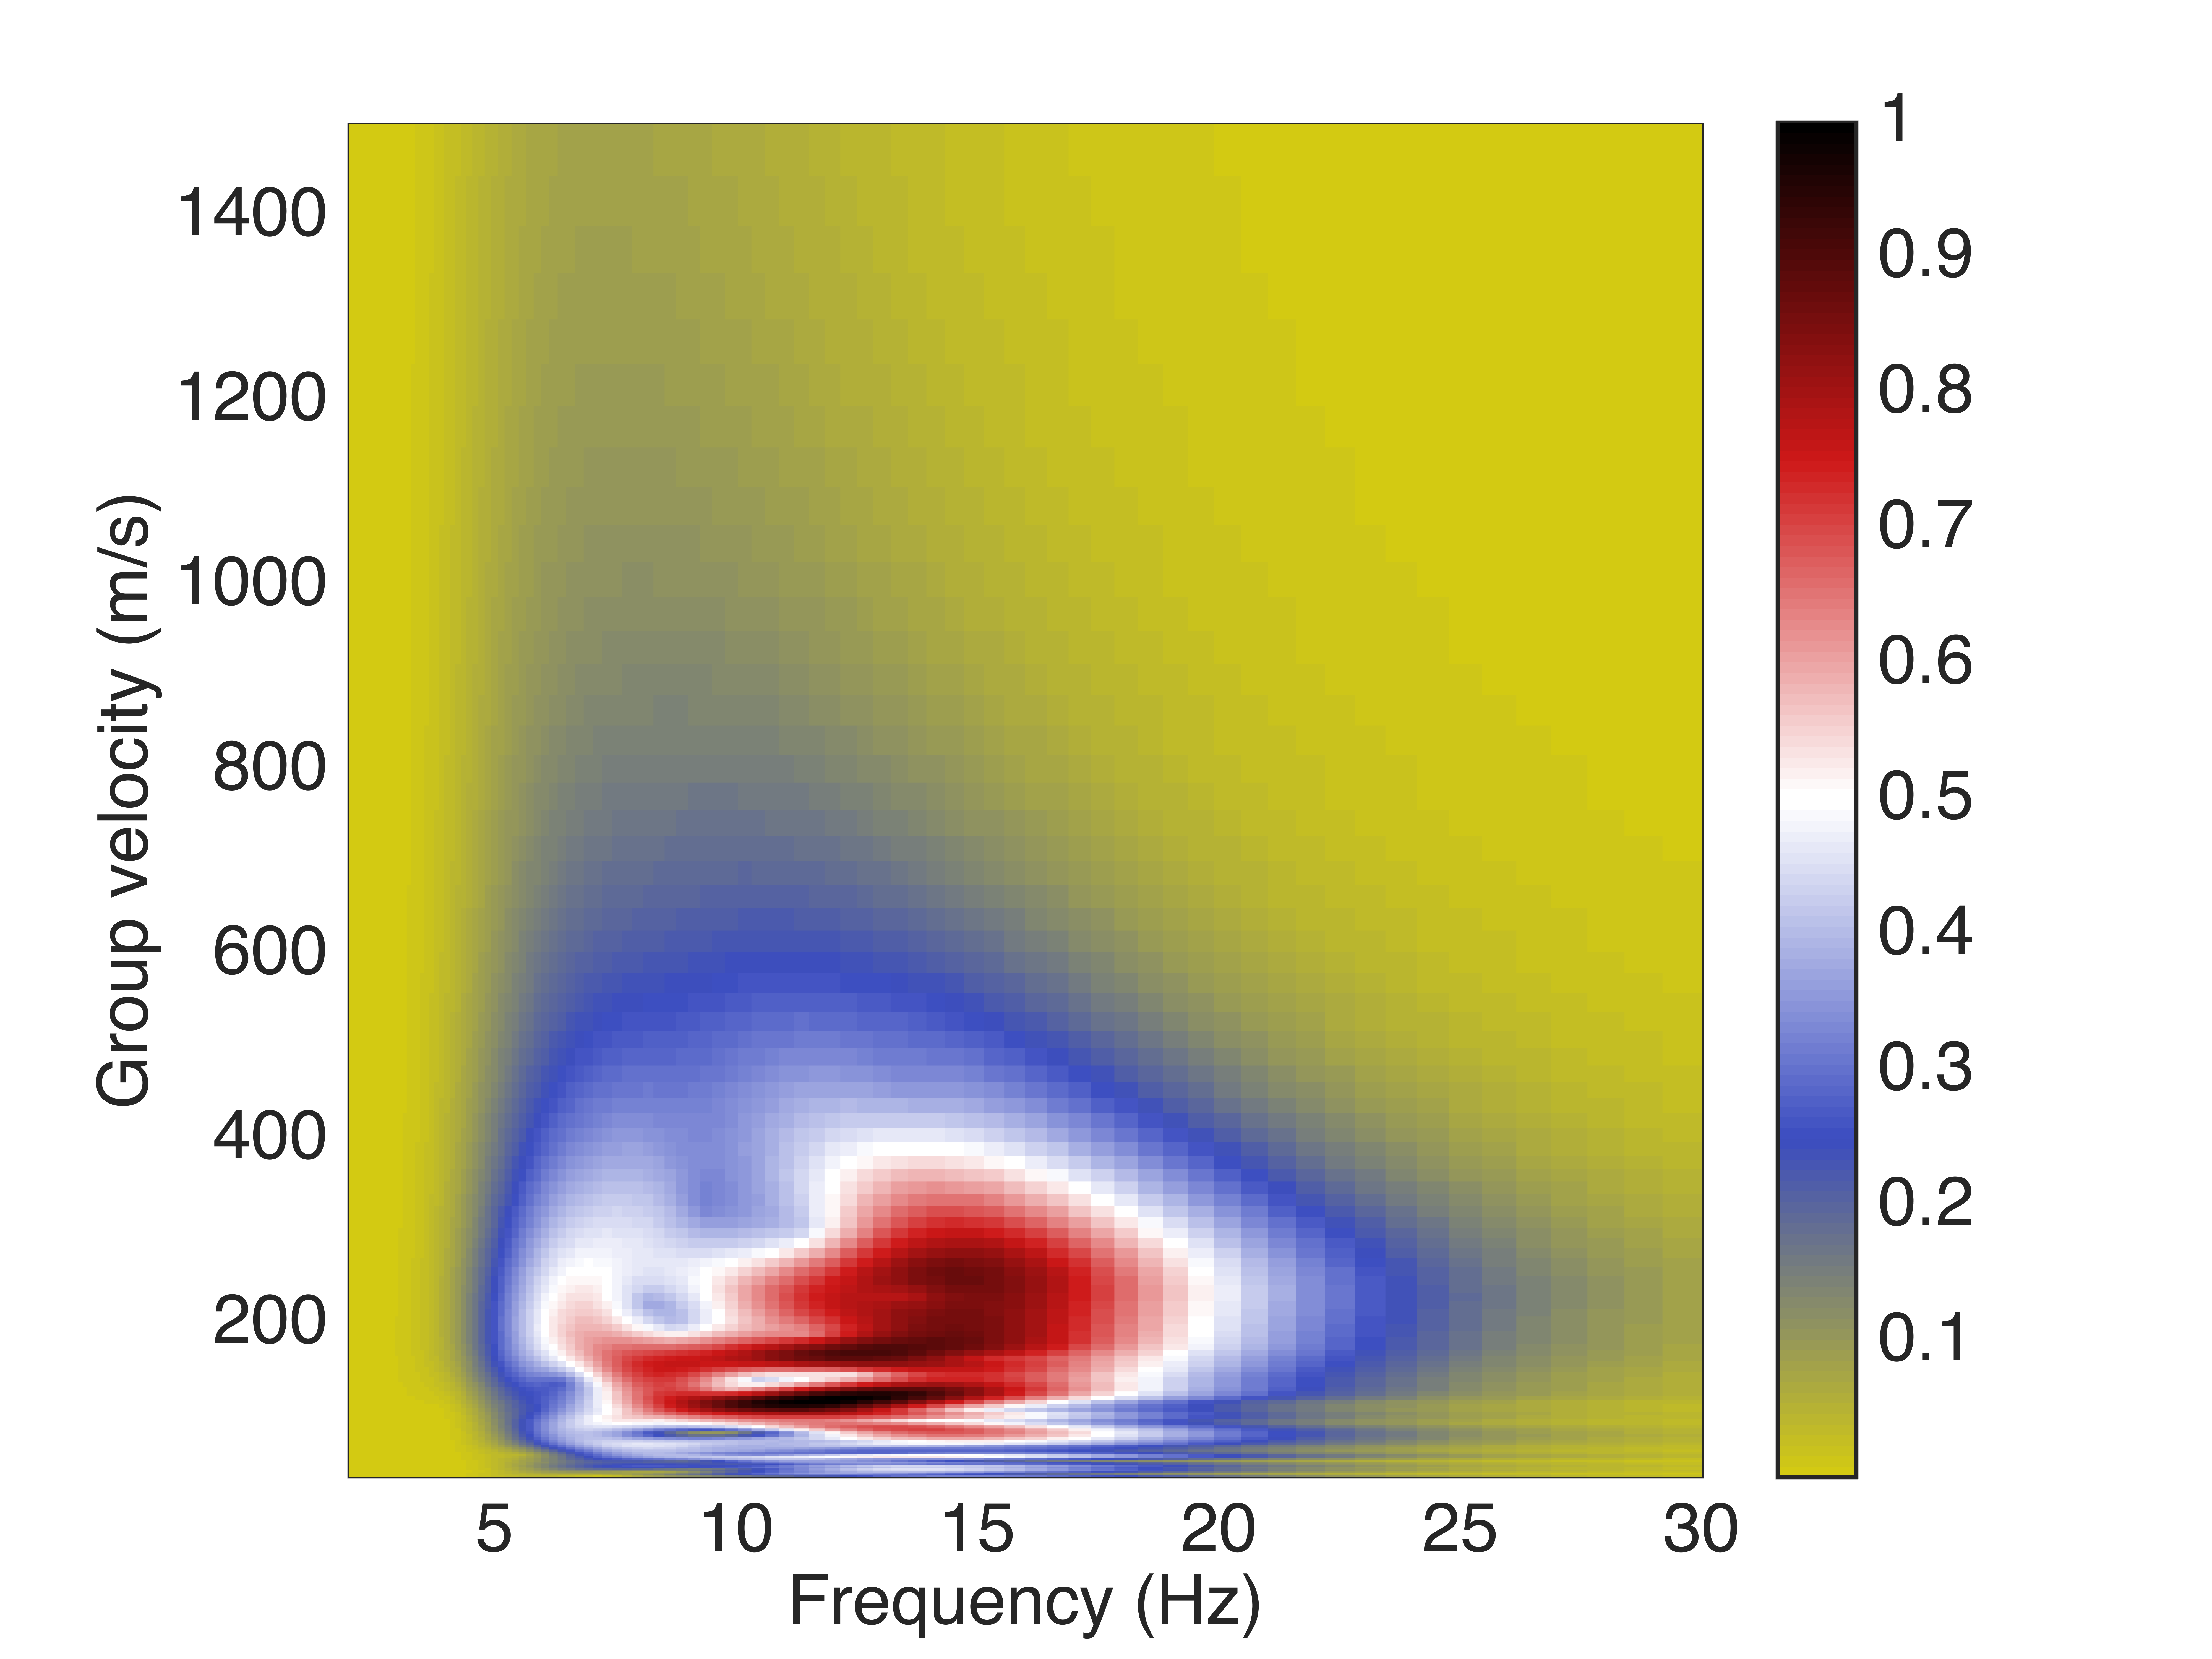
\includegraphics[width=0.9\textwidth]{../pics/C-26-78/group-velocity.png}
}
%--------------------------------------------------------------------
%            group velocity                                                                                   
%--------------------------------------------------------------------
\frame
{
\frametitle{{\bf Group velocity ``medium"}}
\centering
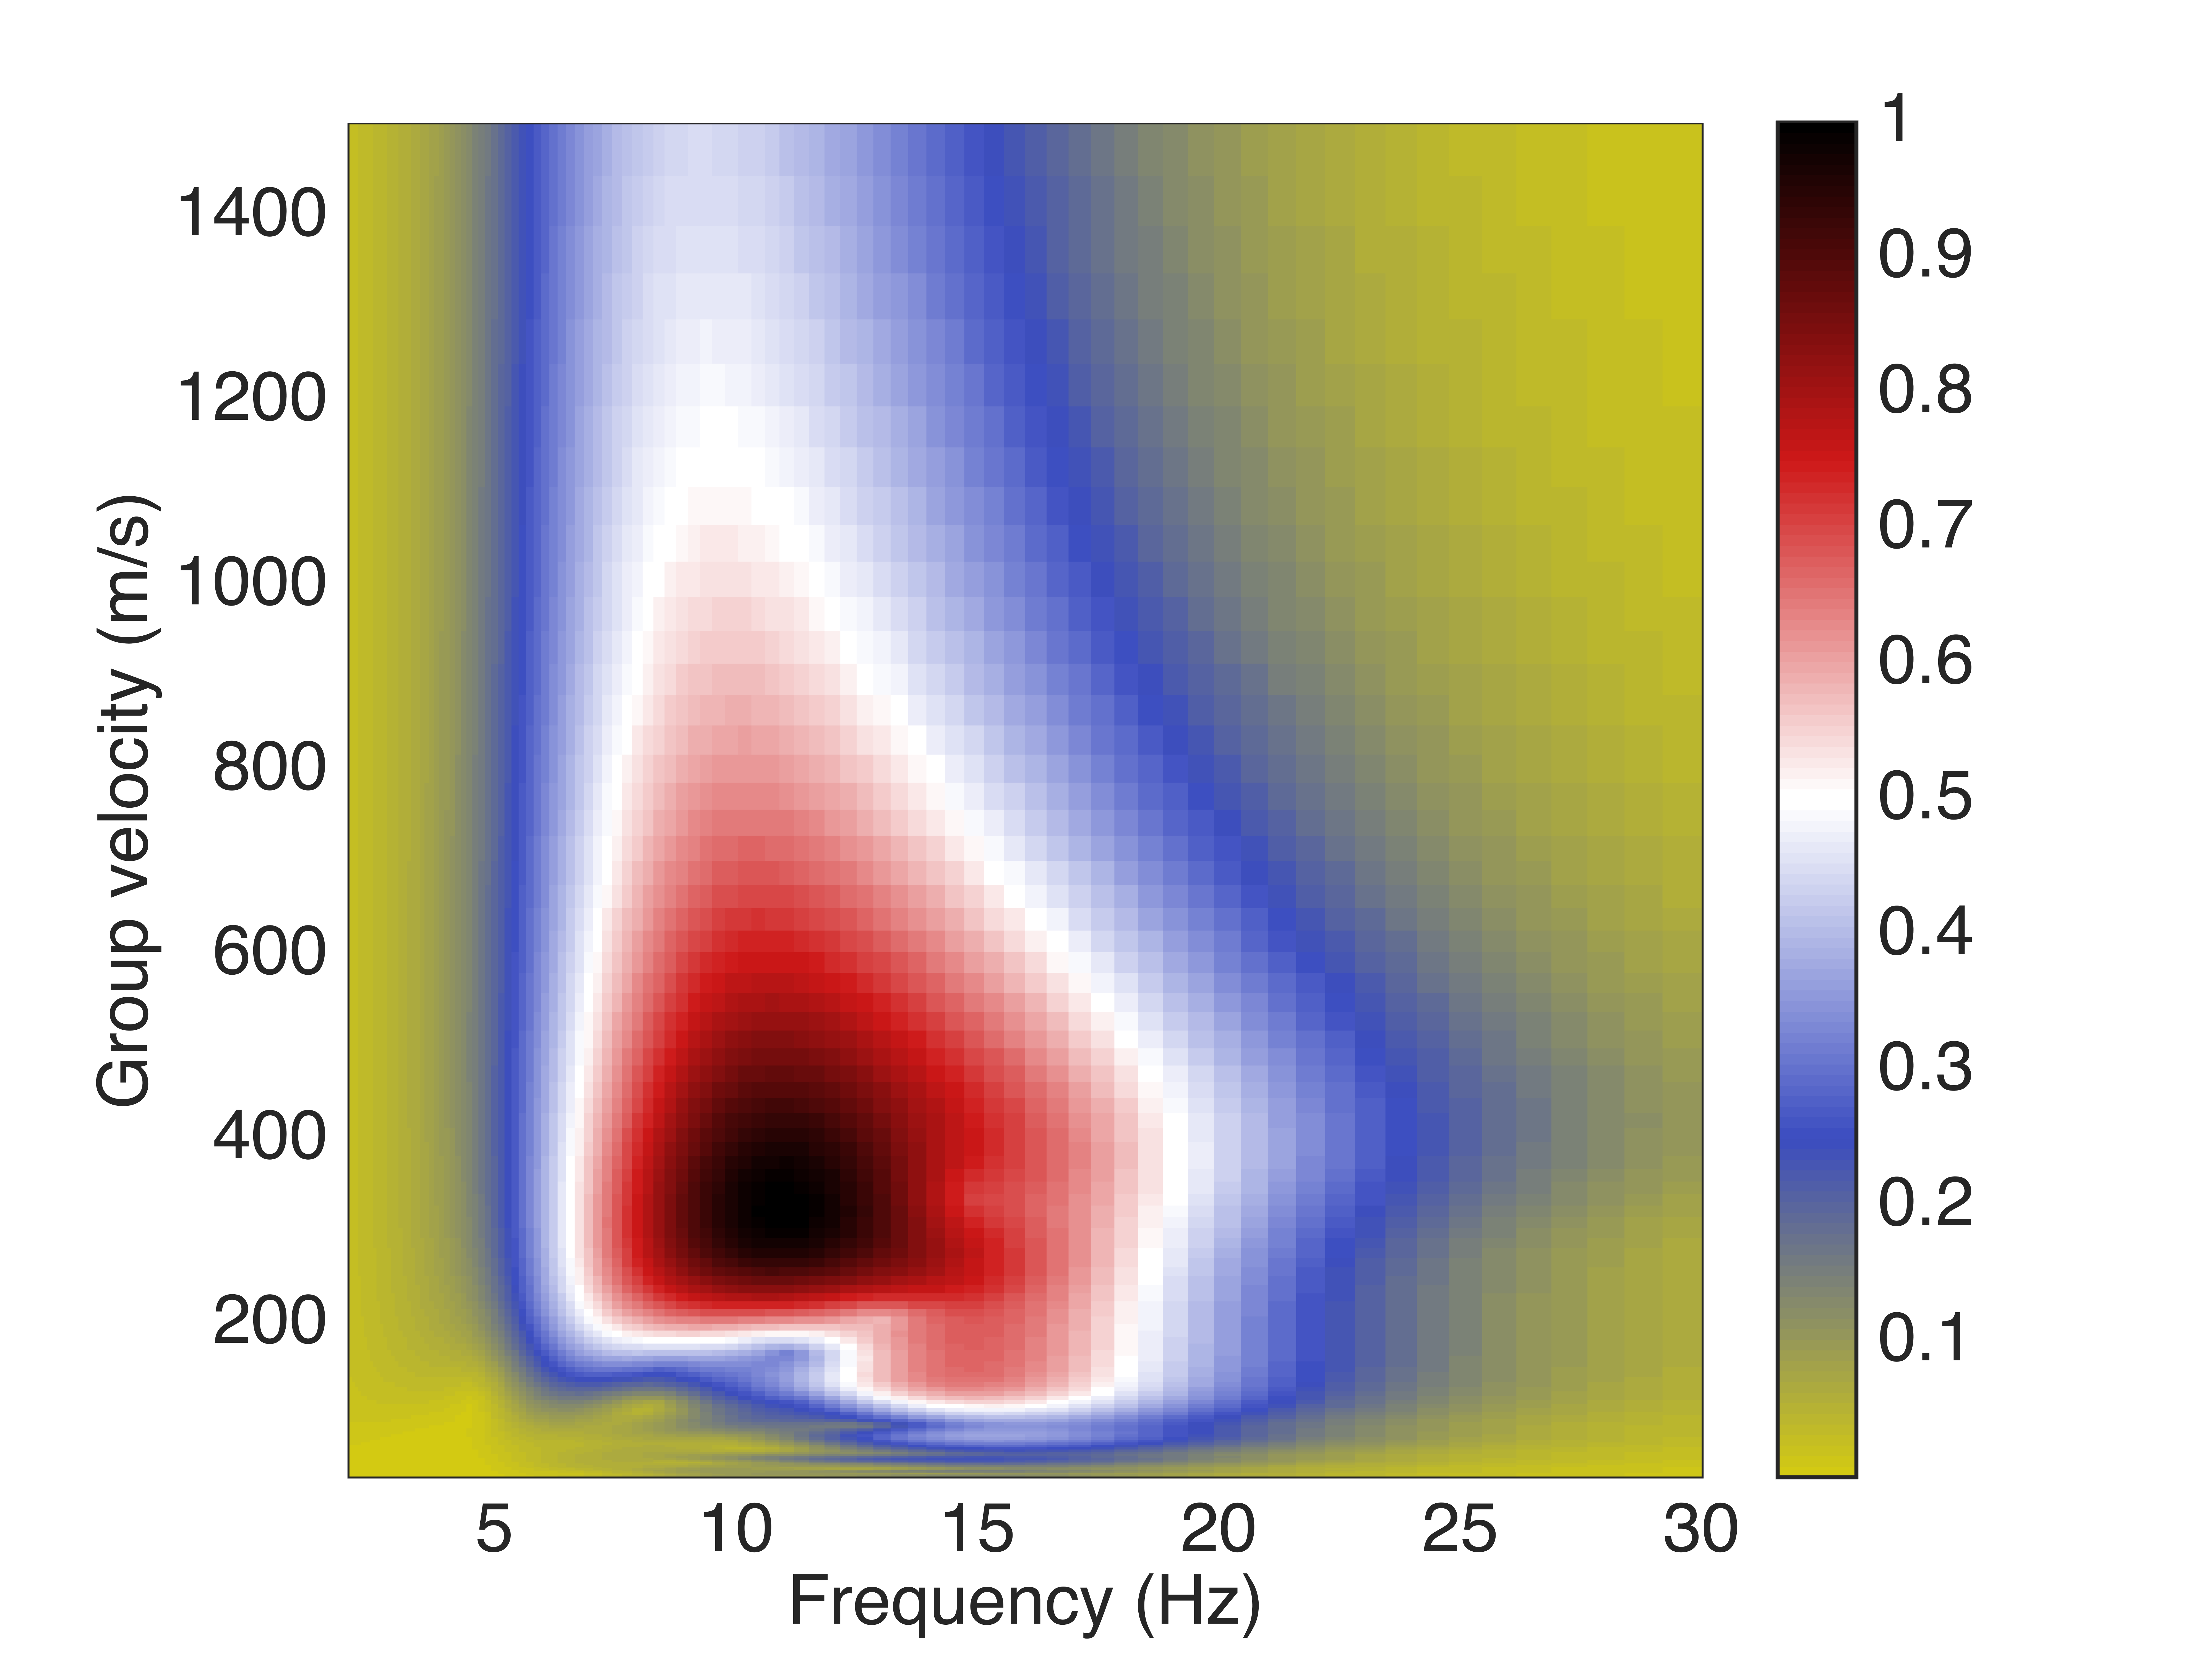
\includegraphics[width=0.9\textwidth]{../pics/C-45-135/group-velocity.png}
}
%--------------------------------------------------------------------
%            group velocity                                                                                   
%--------------------------------------------------------------------
\frame
{
\frametitle{{\bf Group velocity ``large"}}
\centering
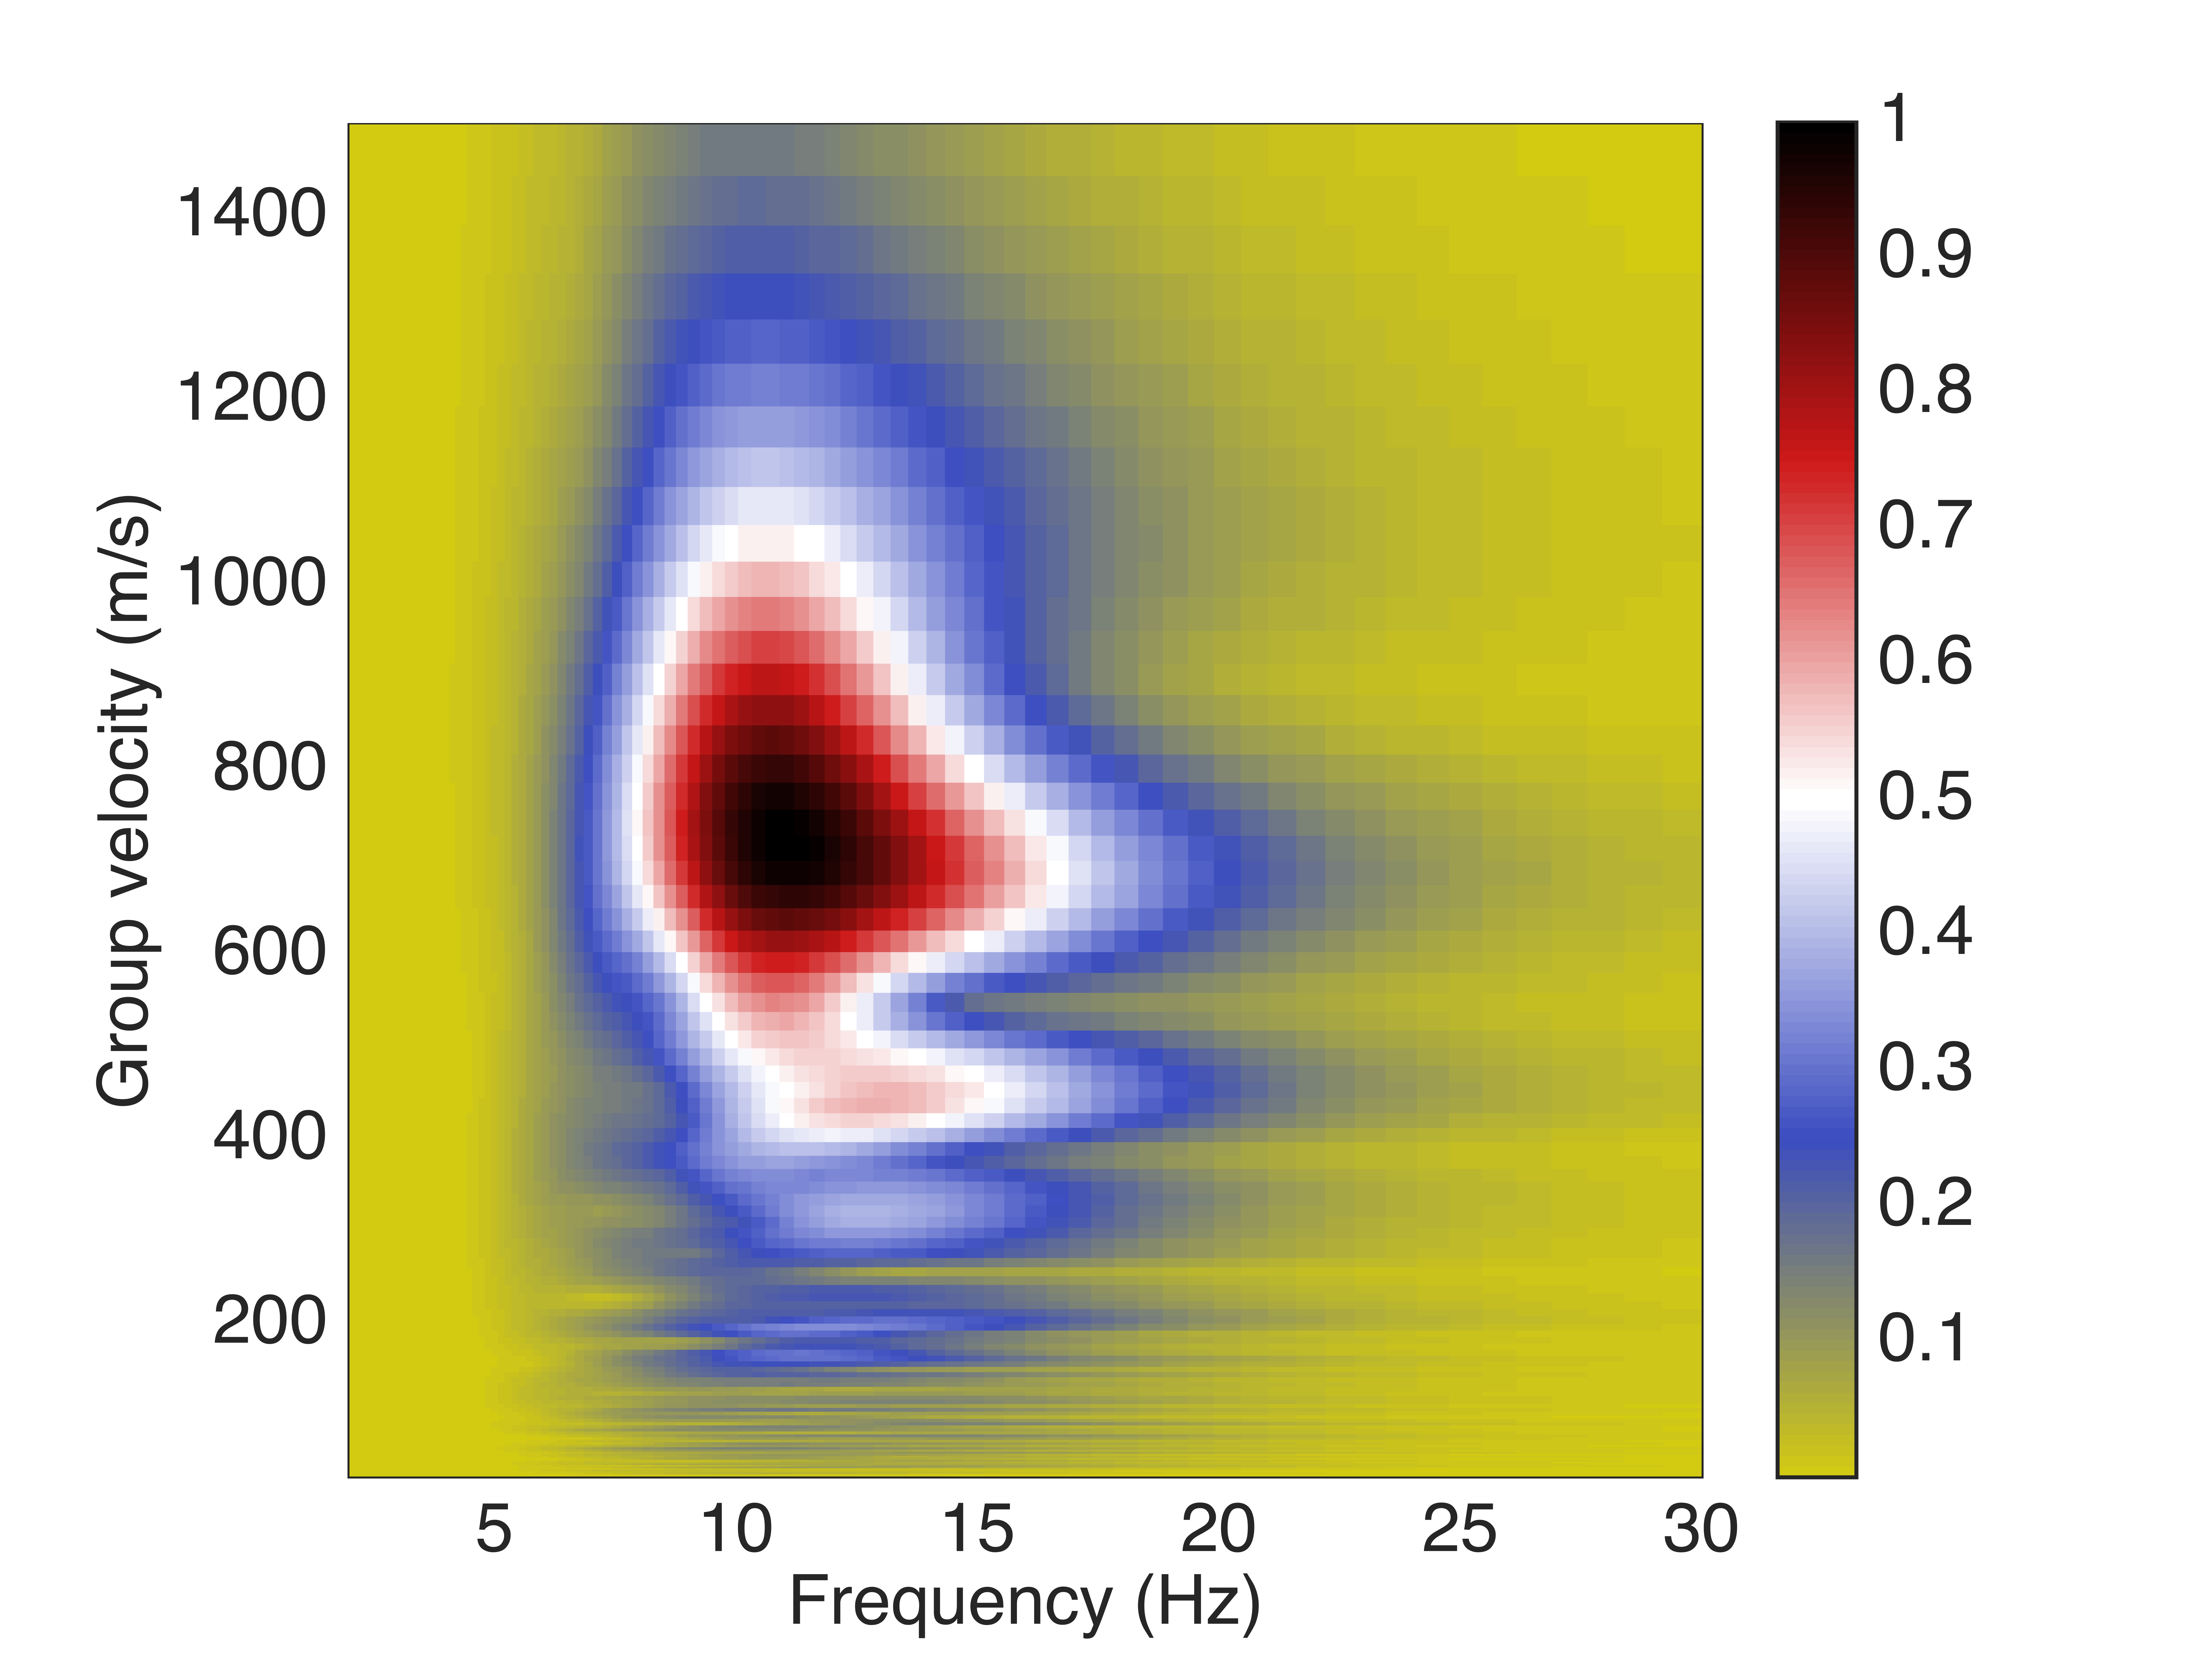
\includegraphics[width=0.9\textwidth]{../pics/C-78-405/group-velocity.png}
}
%--------------------------------------------------------------------
%                                                                                              
%--------------------------------------------------------------------
\frame
{
\frametitle{{\bf Group velocity - all together}}
\centering
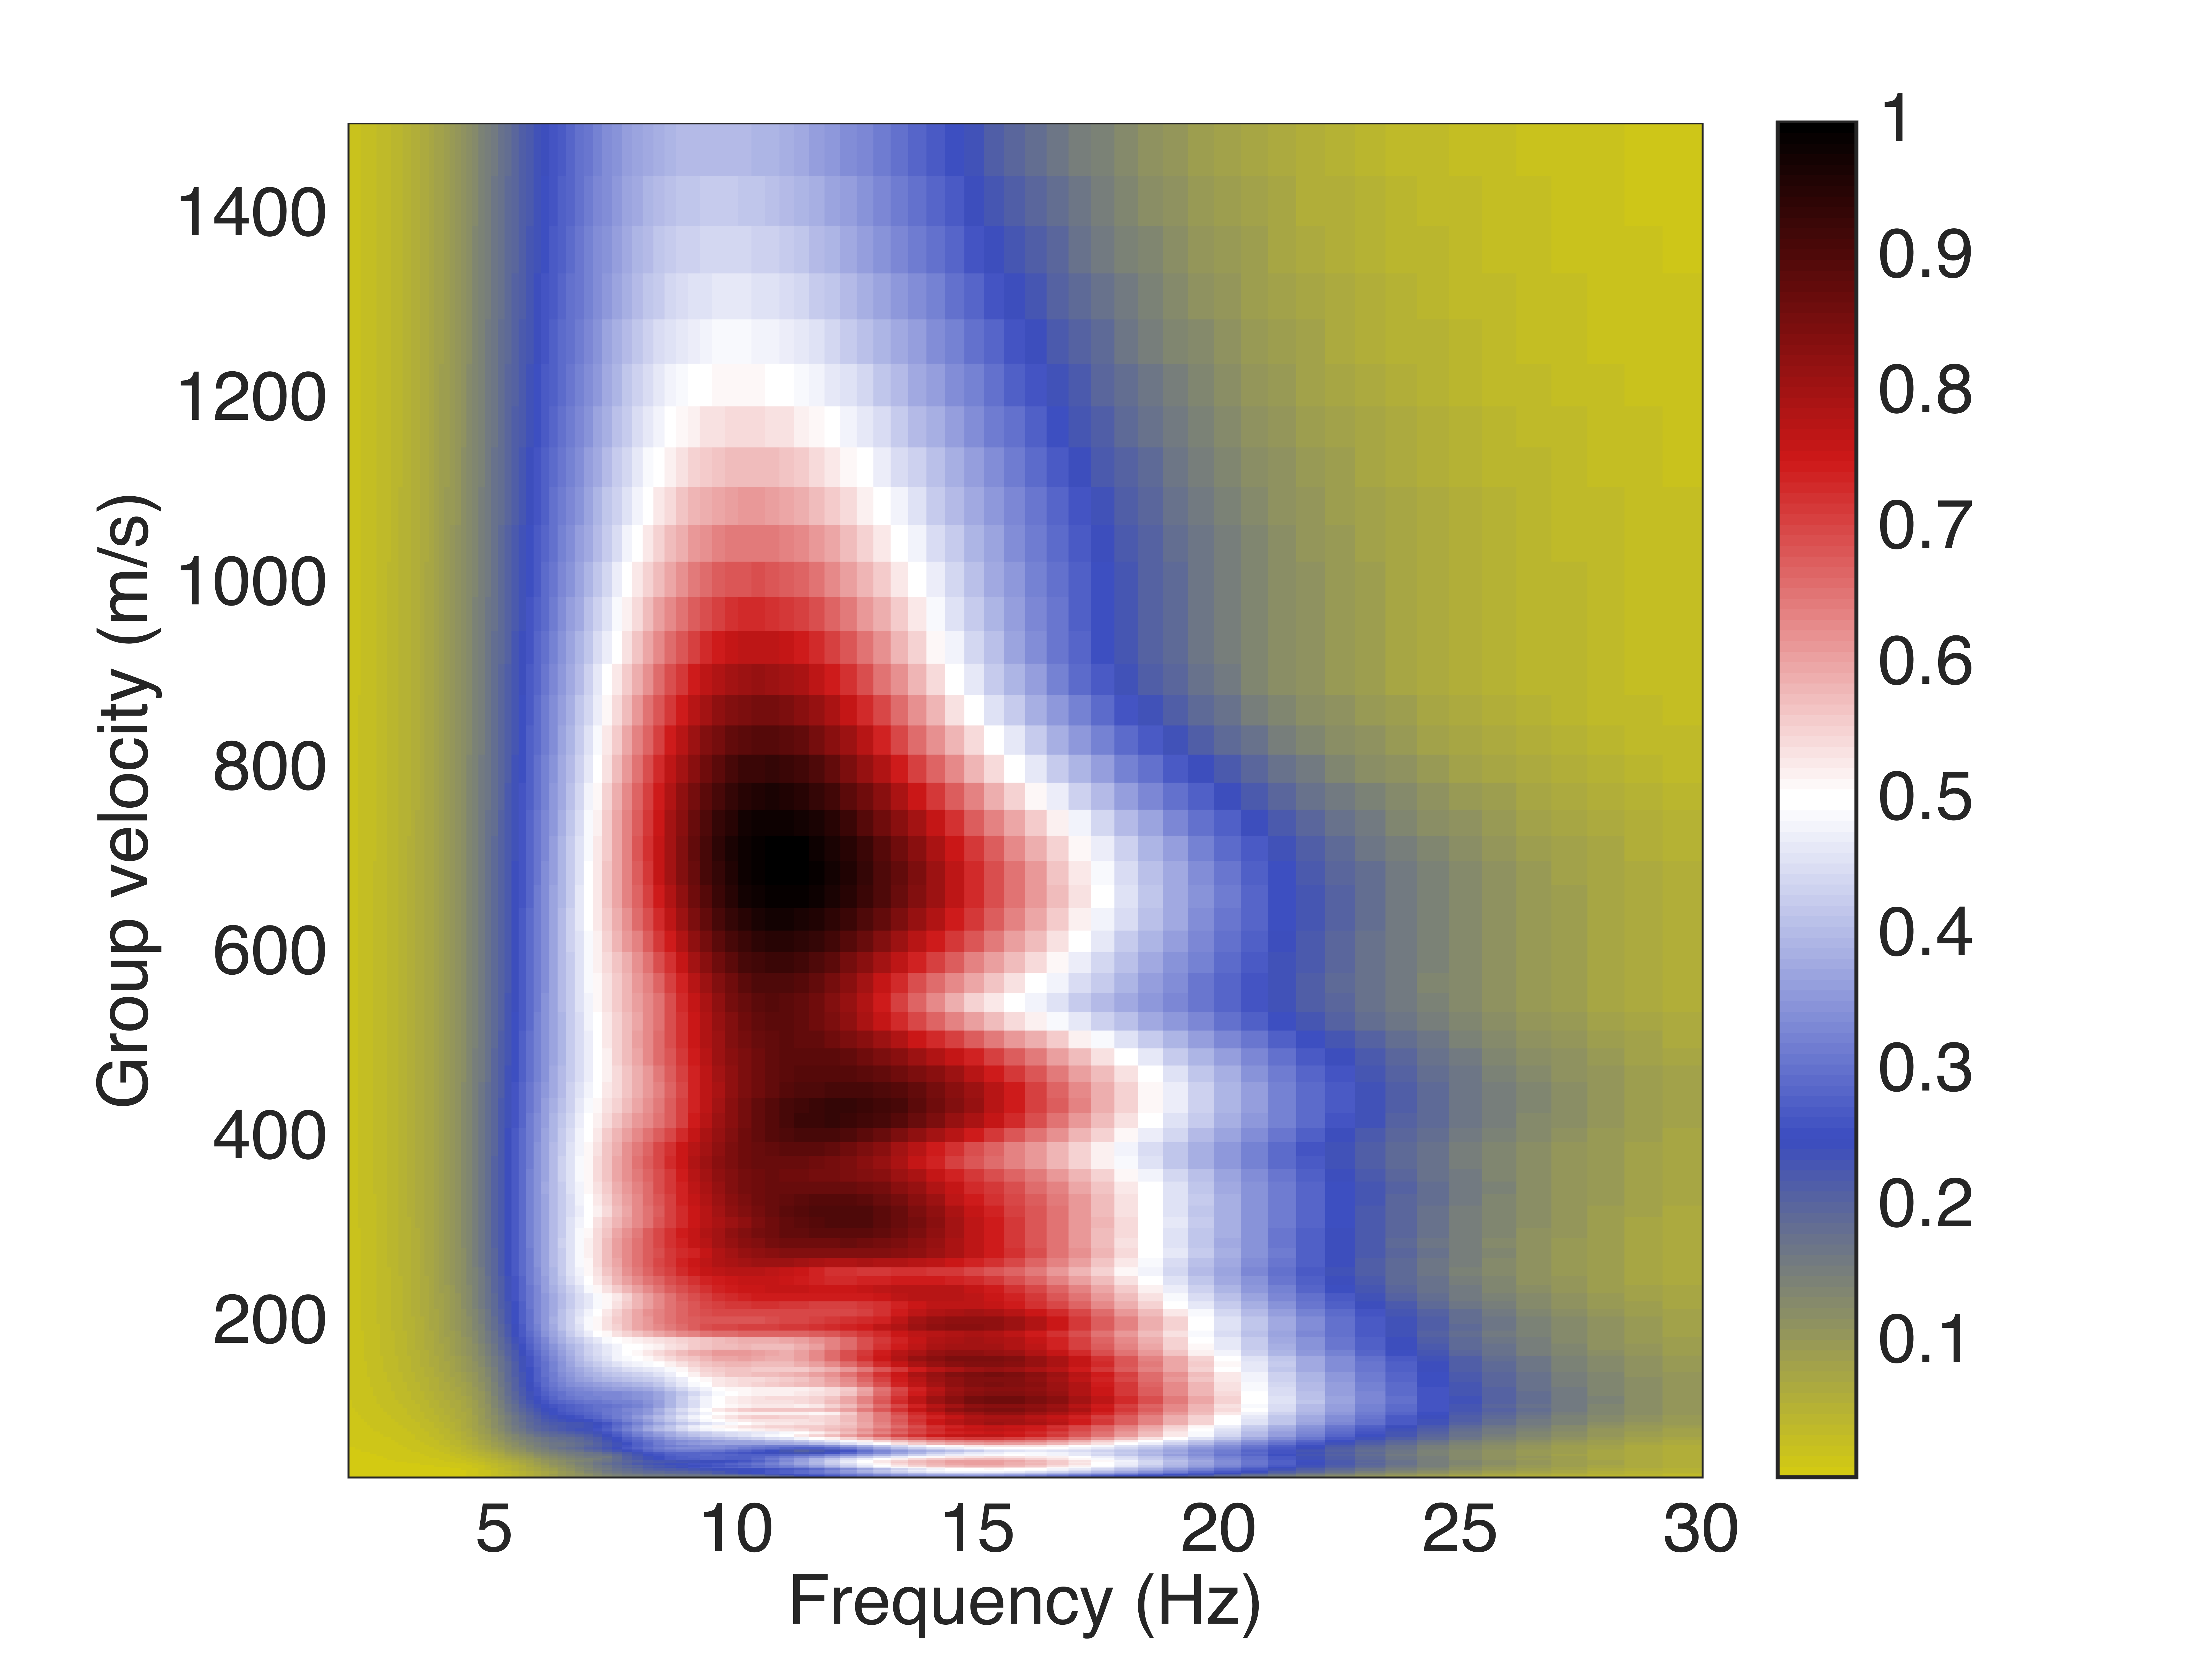
\includegraphics[width=0.9\textwidth]{../pics/group-velocity-onyva.png}
}
%--------------------------------------------------------------------
%                       math                                                                       
%--------------------------------------------------------------------
\frame
{
\frametitle{{\bf Group to phase velocity}}
Let $v_g,v_p,\omega$ and $k$ denote group velocity, phase velocity, angular frequency and wavenumber respectively. We have,
\begin{align*}
v_g &= \partial_k \, \omega, \\
v_p &= \frac{\omega}{k}.
\end{align*}
Let $s$ denote slowness,
\begin{align*}
v_g = \partial_k(k\,v_p) \hspace{2em} \text{or} \hspace{2em} s_g = \partial_\omega(\omega \, s_p)
\end{align*}
and so
\begin{align*}
v_g = k\partial_k \,v_p +  v_p \hspace{2em} \text{or} \hspace{2em} s_g = \omega\partial_\omega \, s_p + s_p.
\end{align*}
Solving these differential equations we have,
\begin{align*}
v_p(\omega) &= \frac{1}{k}\left( k_o\, v_p^o + \int_{k_o}^{k} v_g(k)\;{\rm d}k \right) 
\hspace{2em} 
\text{or} \\
s_p(\omega) &= \frac{1}{\omega}\left( \omega_o\, s_p^o + \int_{\omega_o}^{\omega} s_g(\omega)\;{\rm d}\omega \right).
\end{align*}
}
%--------------------------------------------------------------------
%                                                                                              
%--------------------------------------------------------------------
\frame
{
\frametitle{{\bf Phase velocity - Idea 1}}
\centering
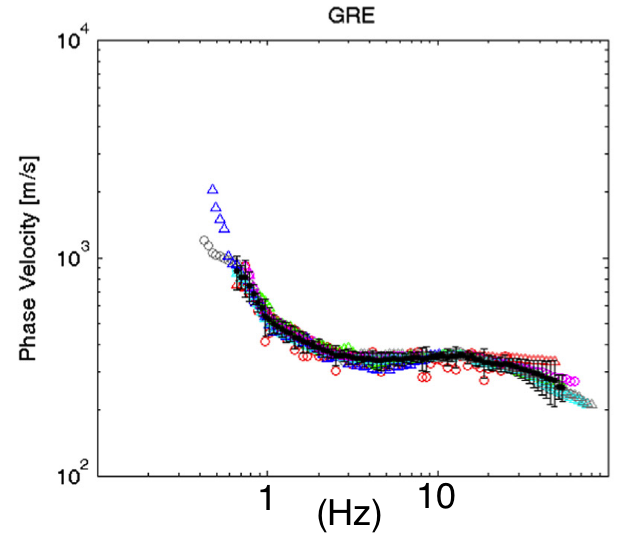
\includegraphics[width=0.45\textwidth]{../pics/phase-vel.png}~
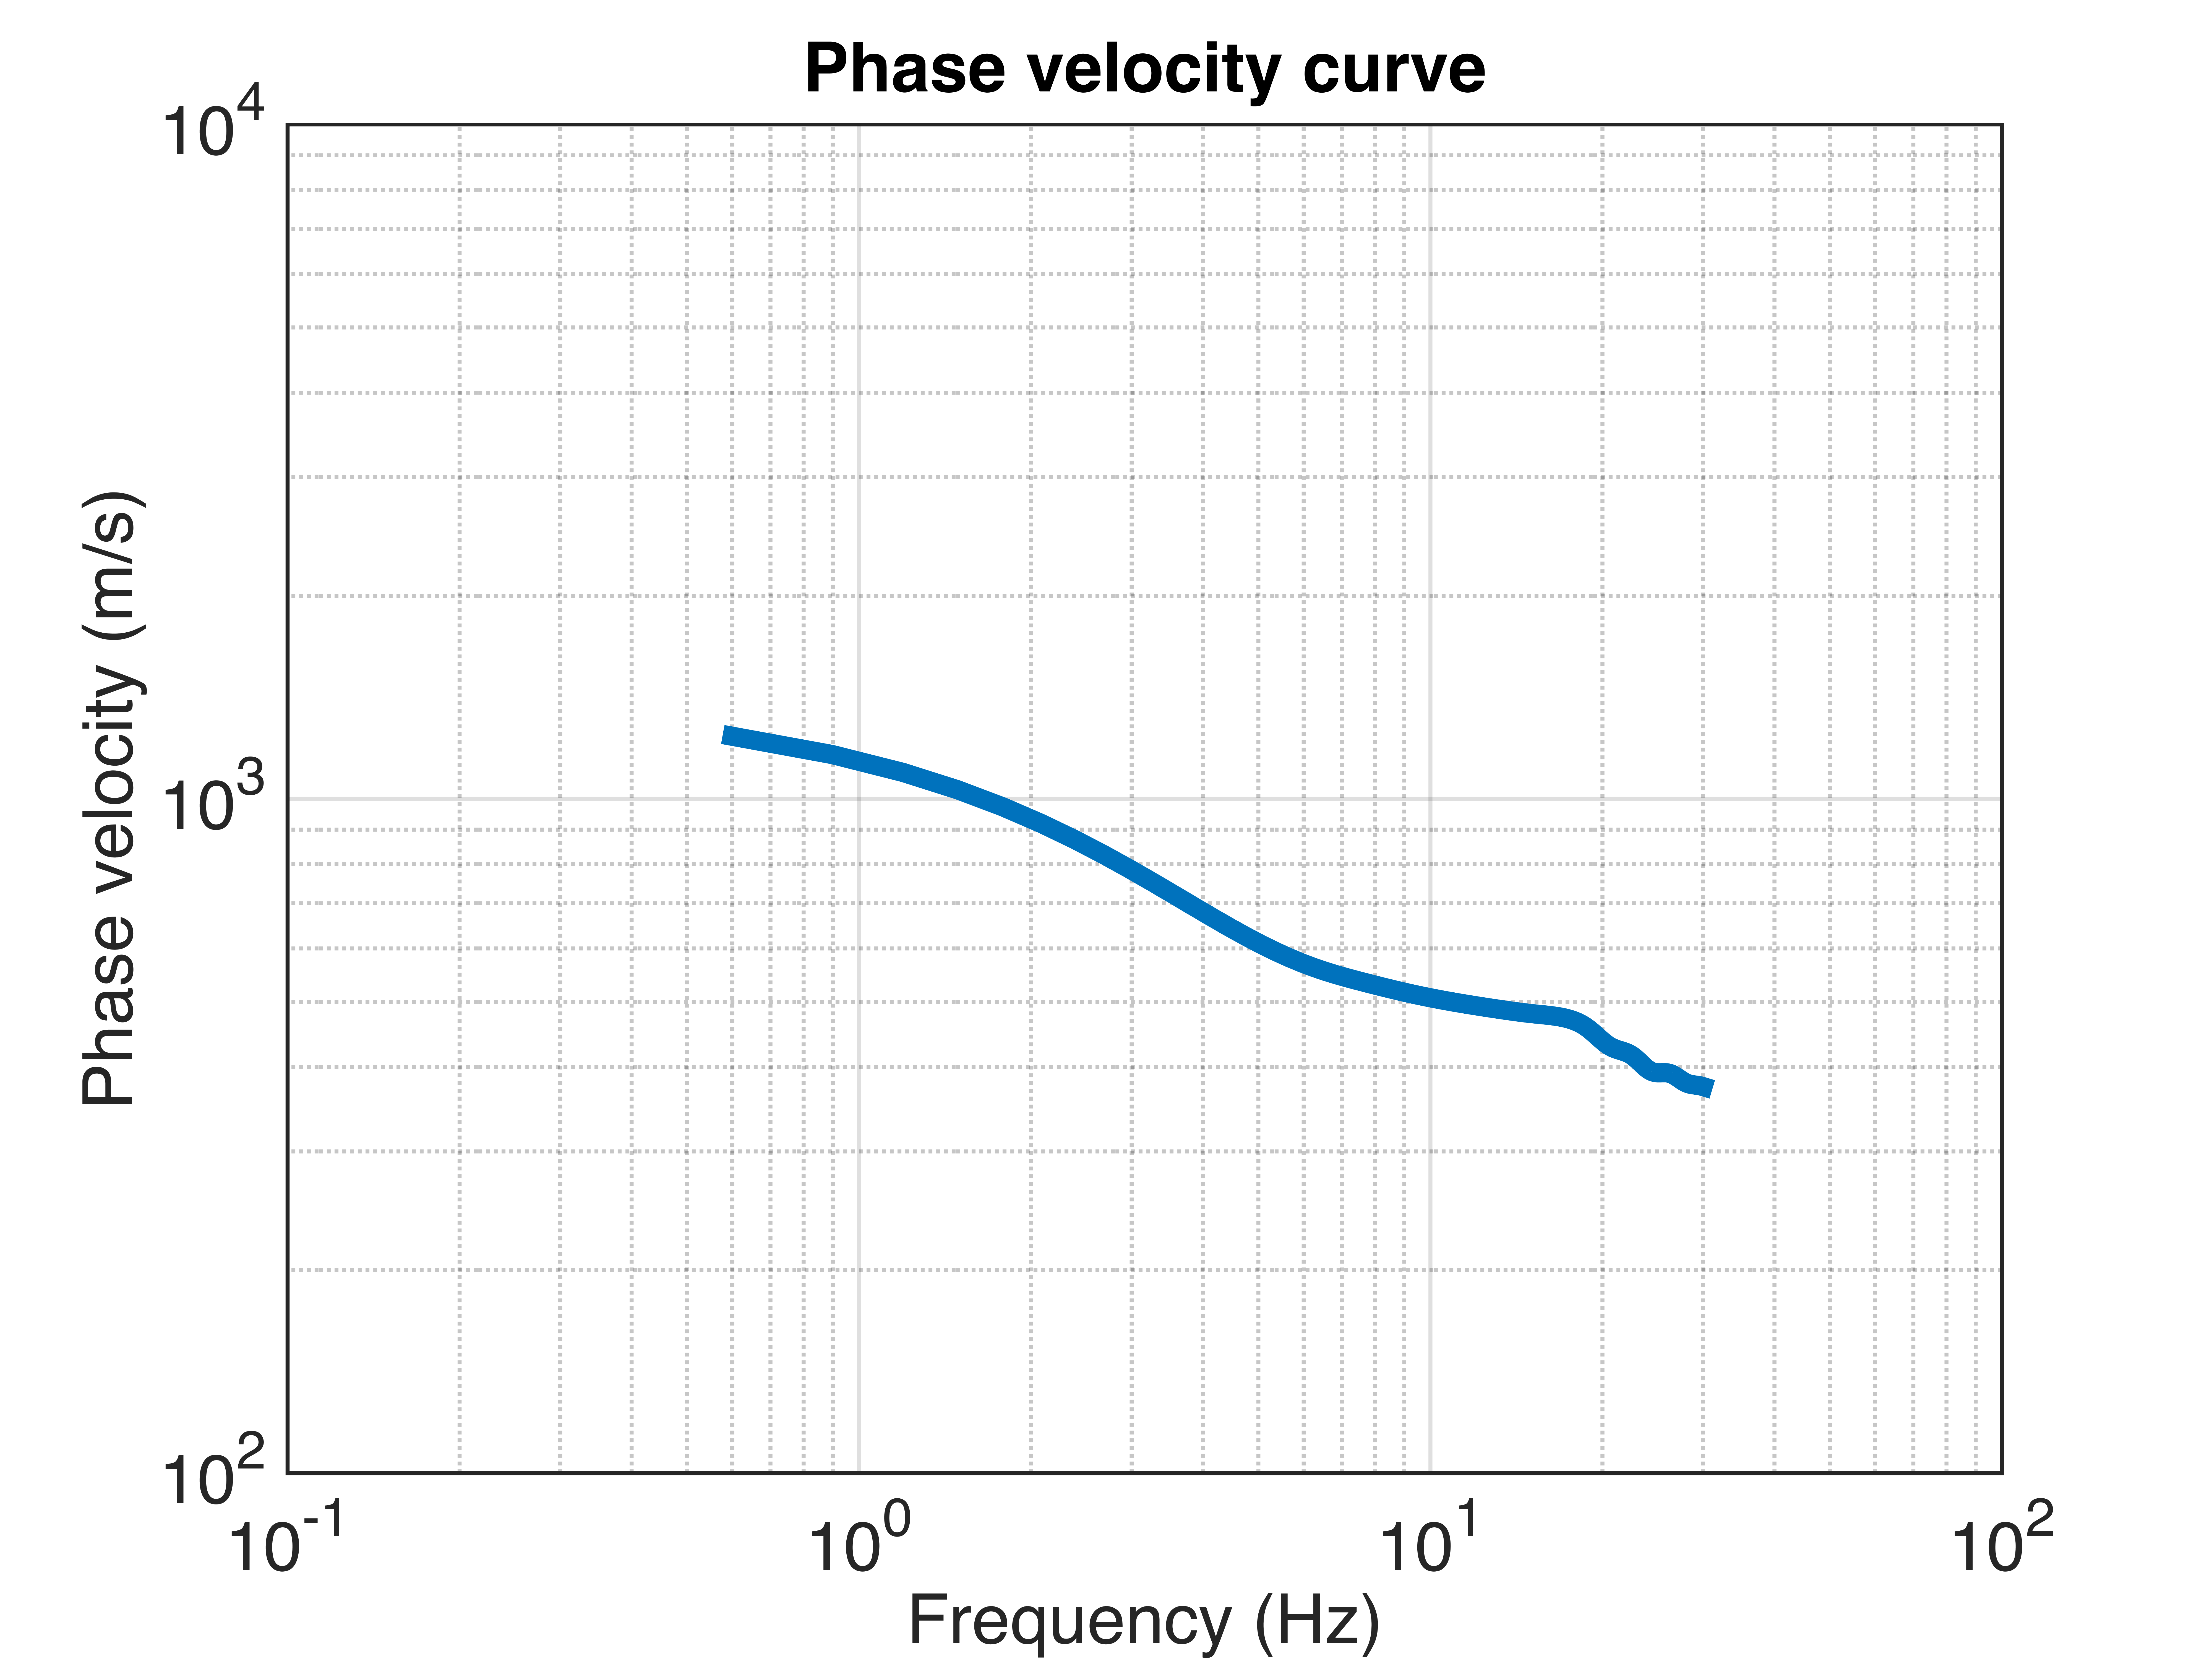
\includegraphics[width=0.5\textwidth]{../pics/phase-vel-onyva.png}
\vfill
\flushleft
Garofalo et al, 2016
}
%--------------------------------------------------------------------
%                                                                                              
%--------------------------------------------------------------------
\frame
{
\frametitle{{\bf Phase velocity - Idea 2}}
\centering
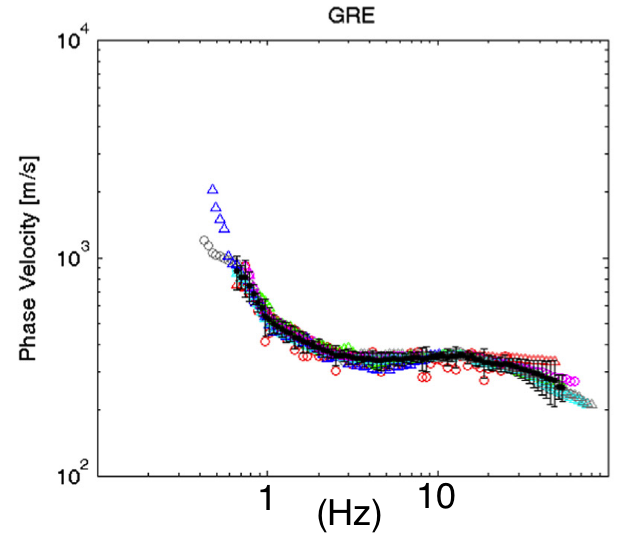
\includegraphics[width=0.45\textwidth]{../pics/phase-vel.png}~
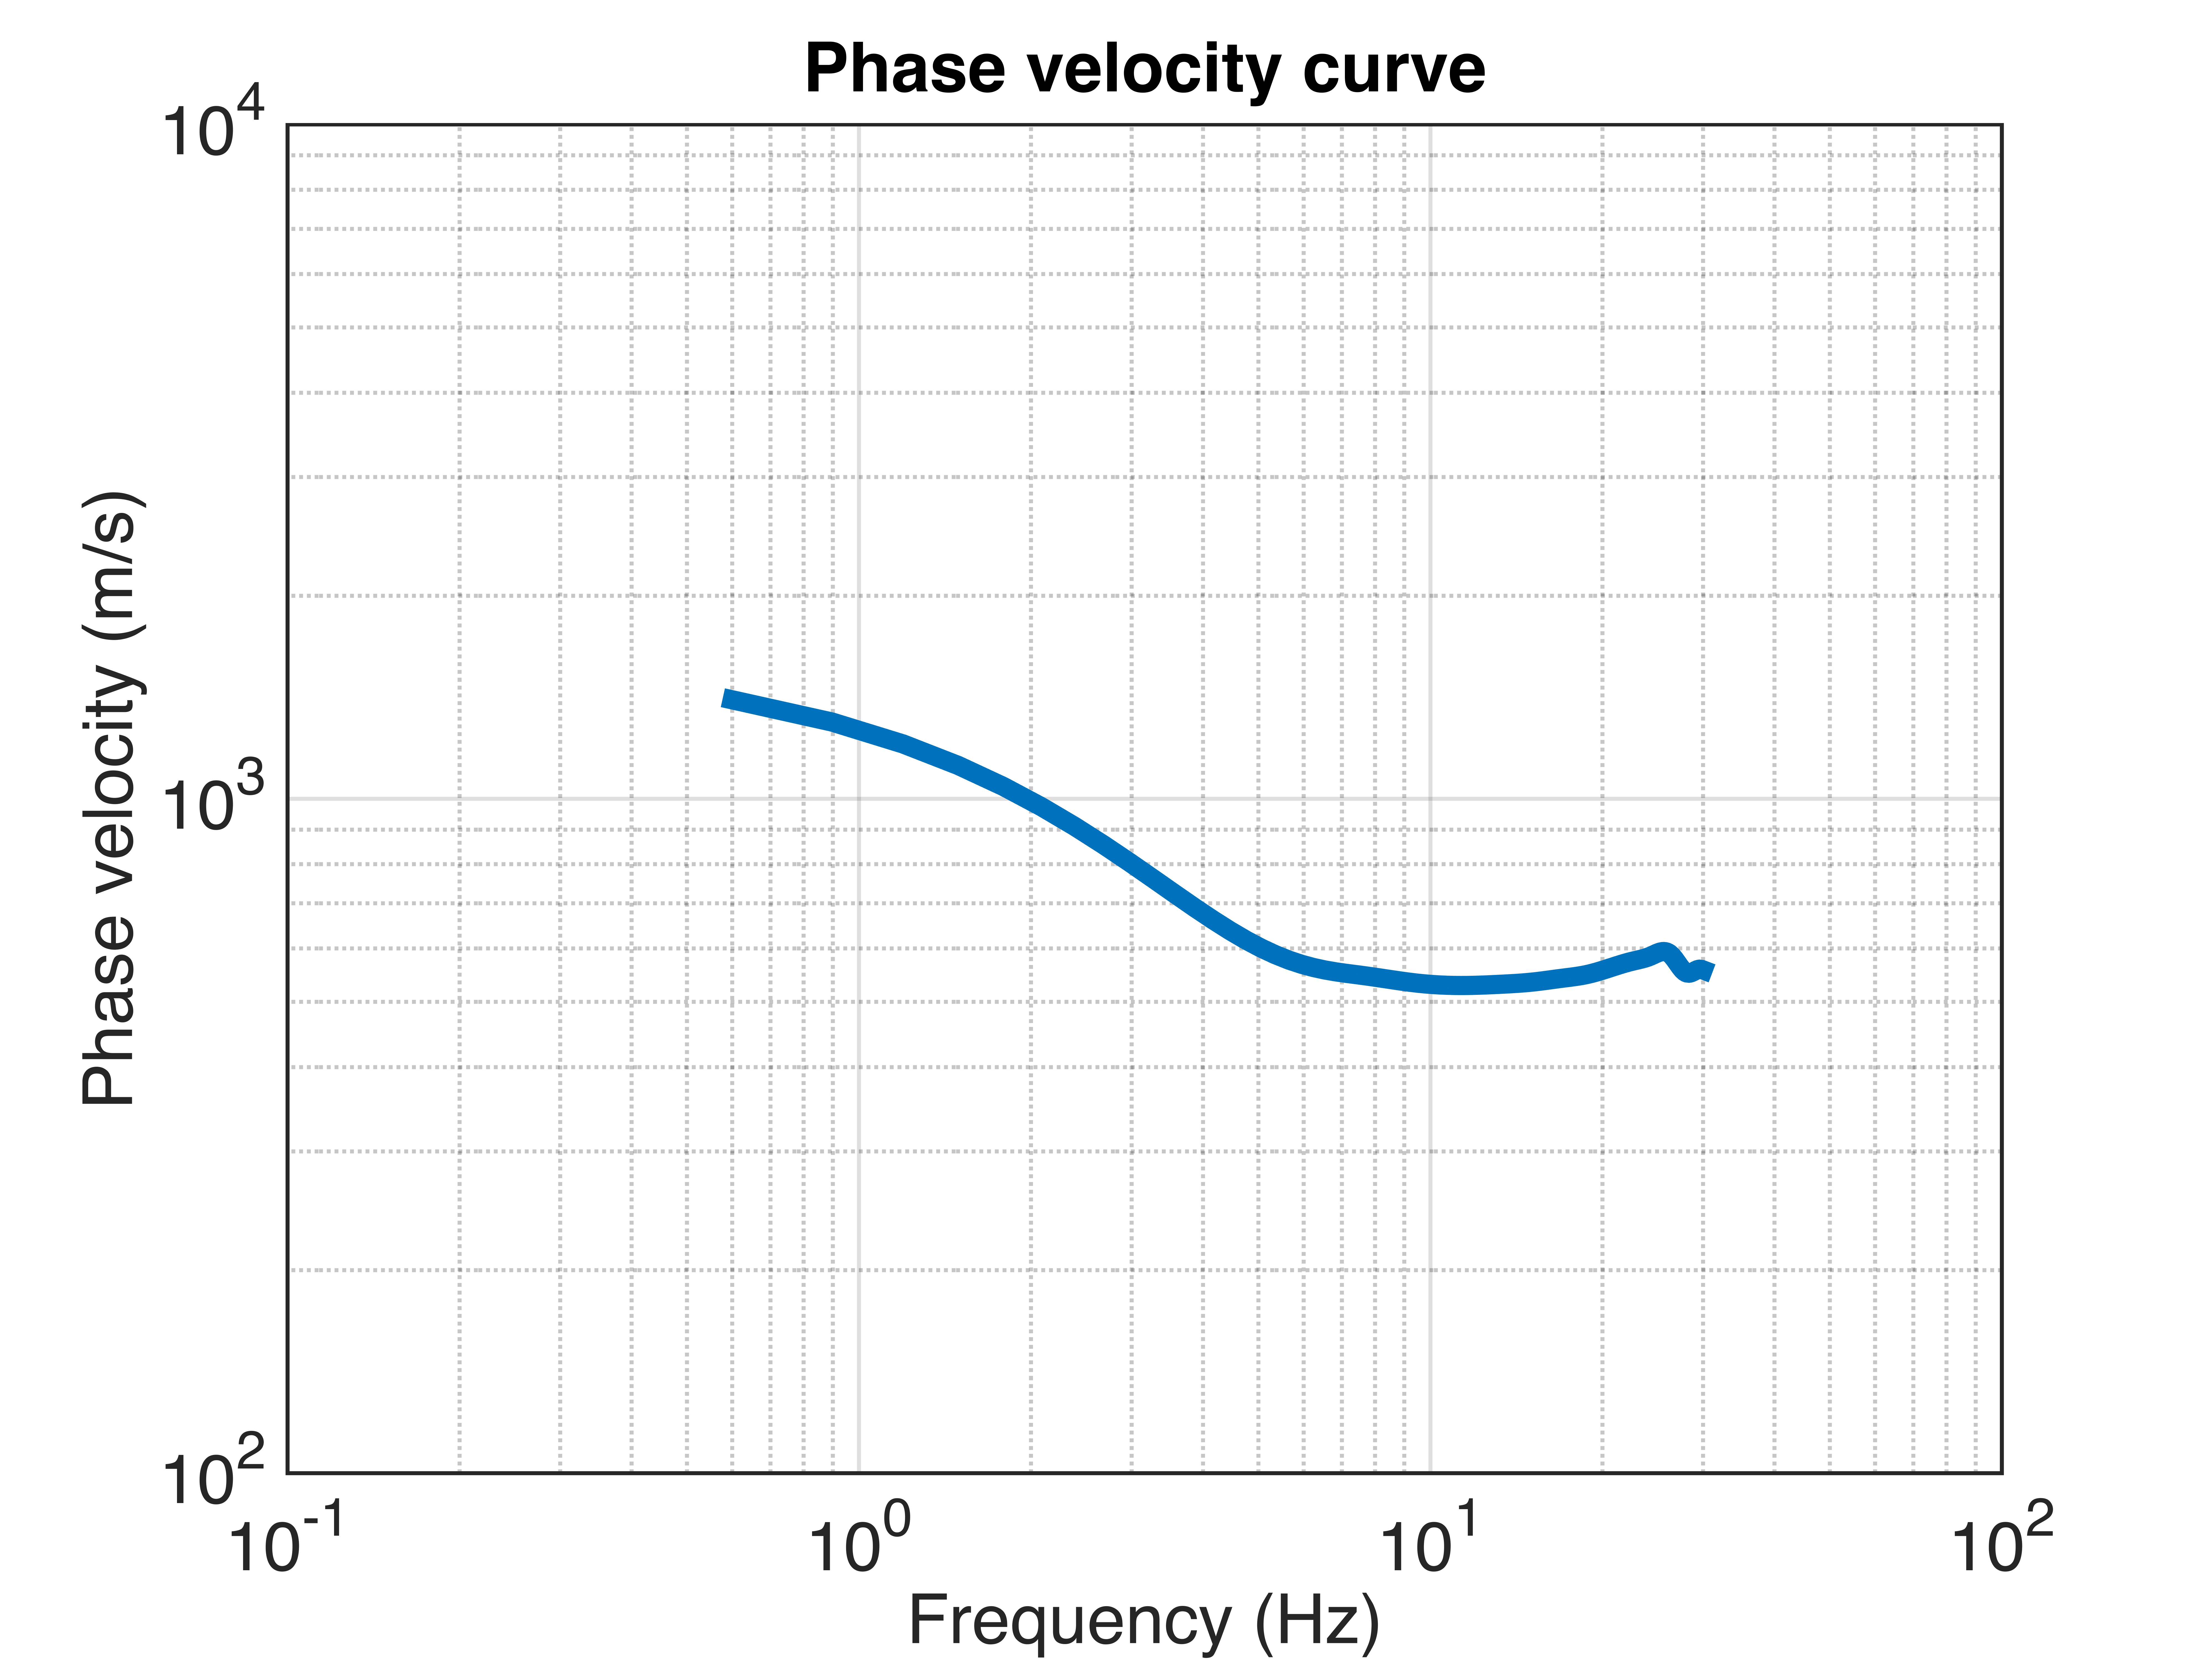
\includegraphics[width=0.5\textwidth]{../pics/phase-vel-vamos.png}
\vfill
\flushleft
Garofalo et al, 2016
}
%--------------------------------------------------------------------
%                                                                                              
%--------------------------------------------------------------------
\frame
{
\frametitle{{\bf Shot gather - Idea 1}}
\centering
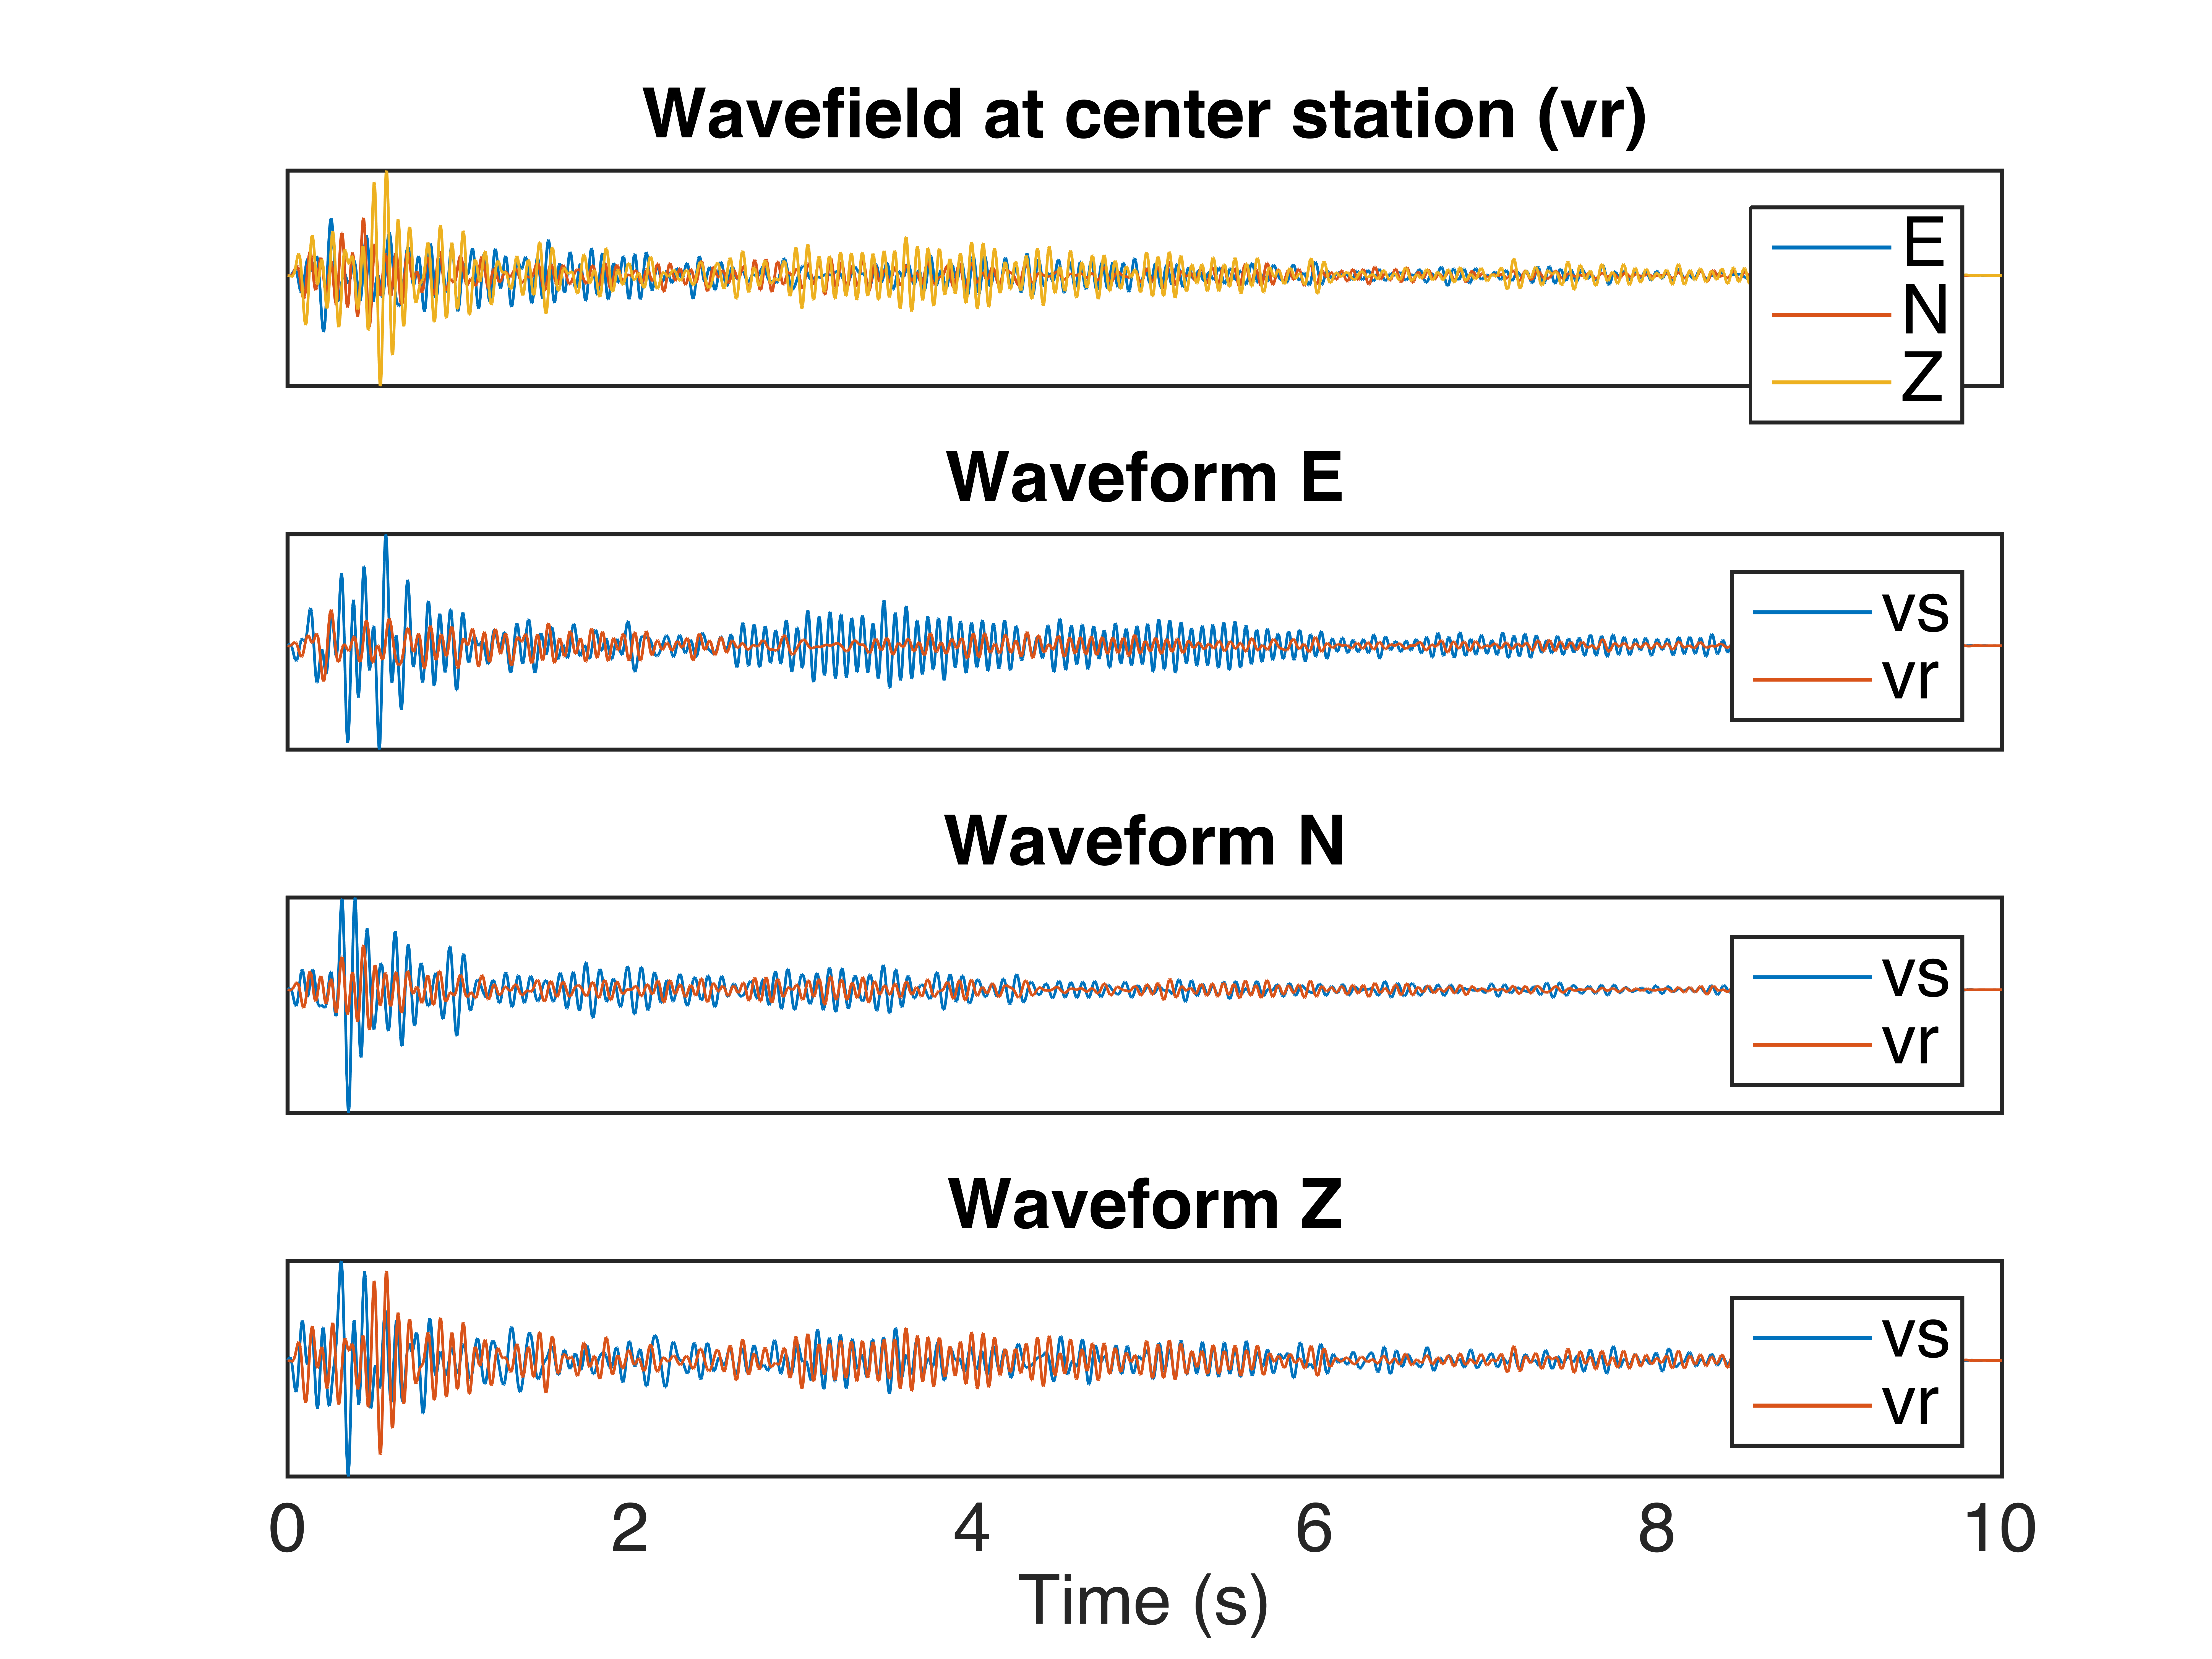
\includegraphics[width=\textwidth]{../pics/C-26-78/vr.png}
}
%--------------------------------------------------------------------
%                                                                                              
%--------------------------------------------------------------------
\frame
{
\frametitle{{\bf Shot gather - Idea 2}}
\centering
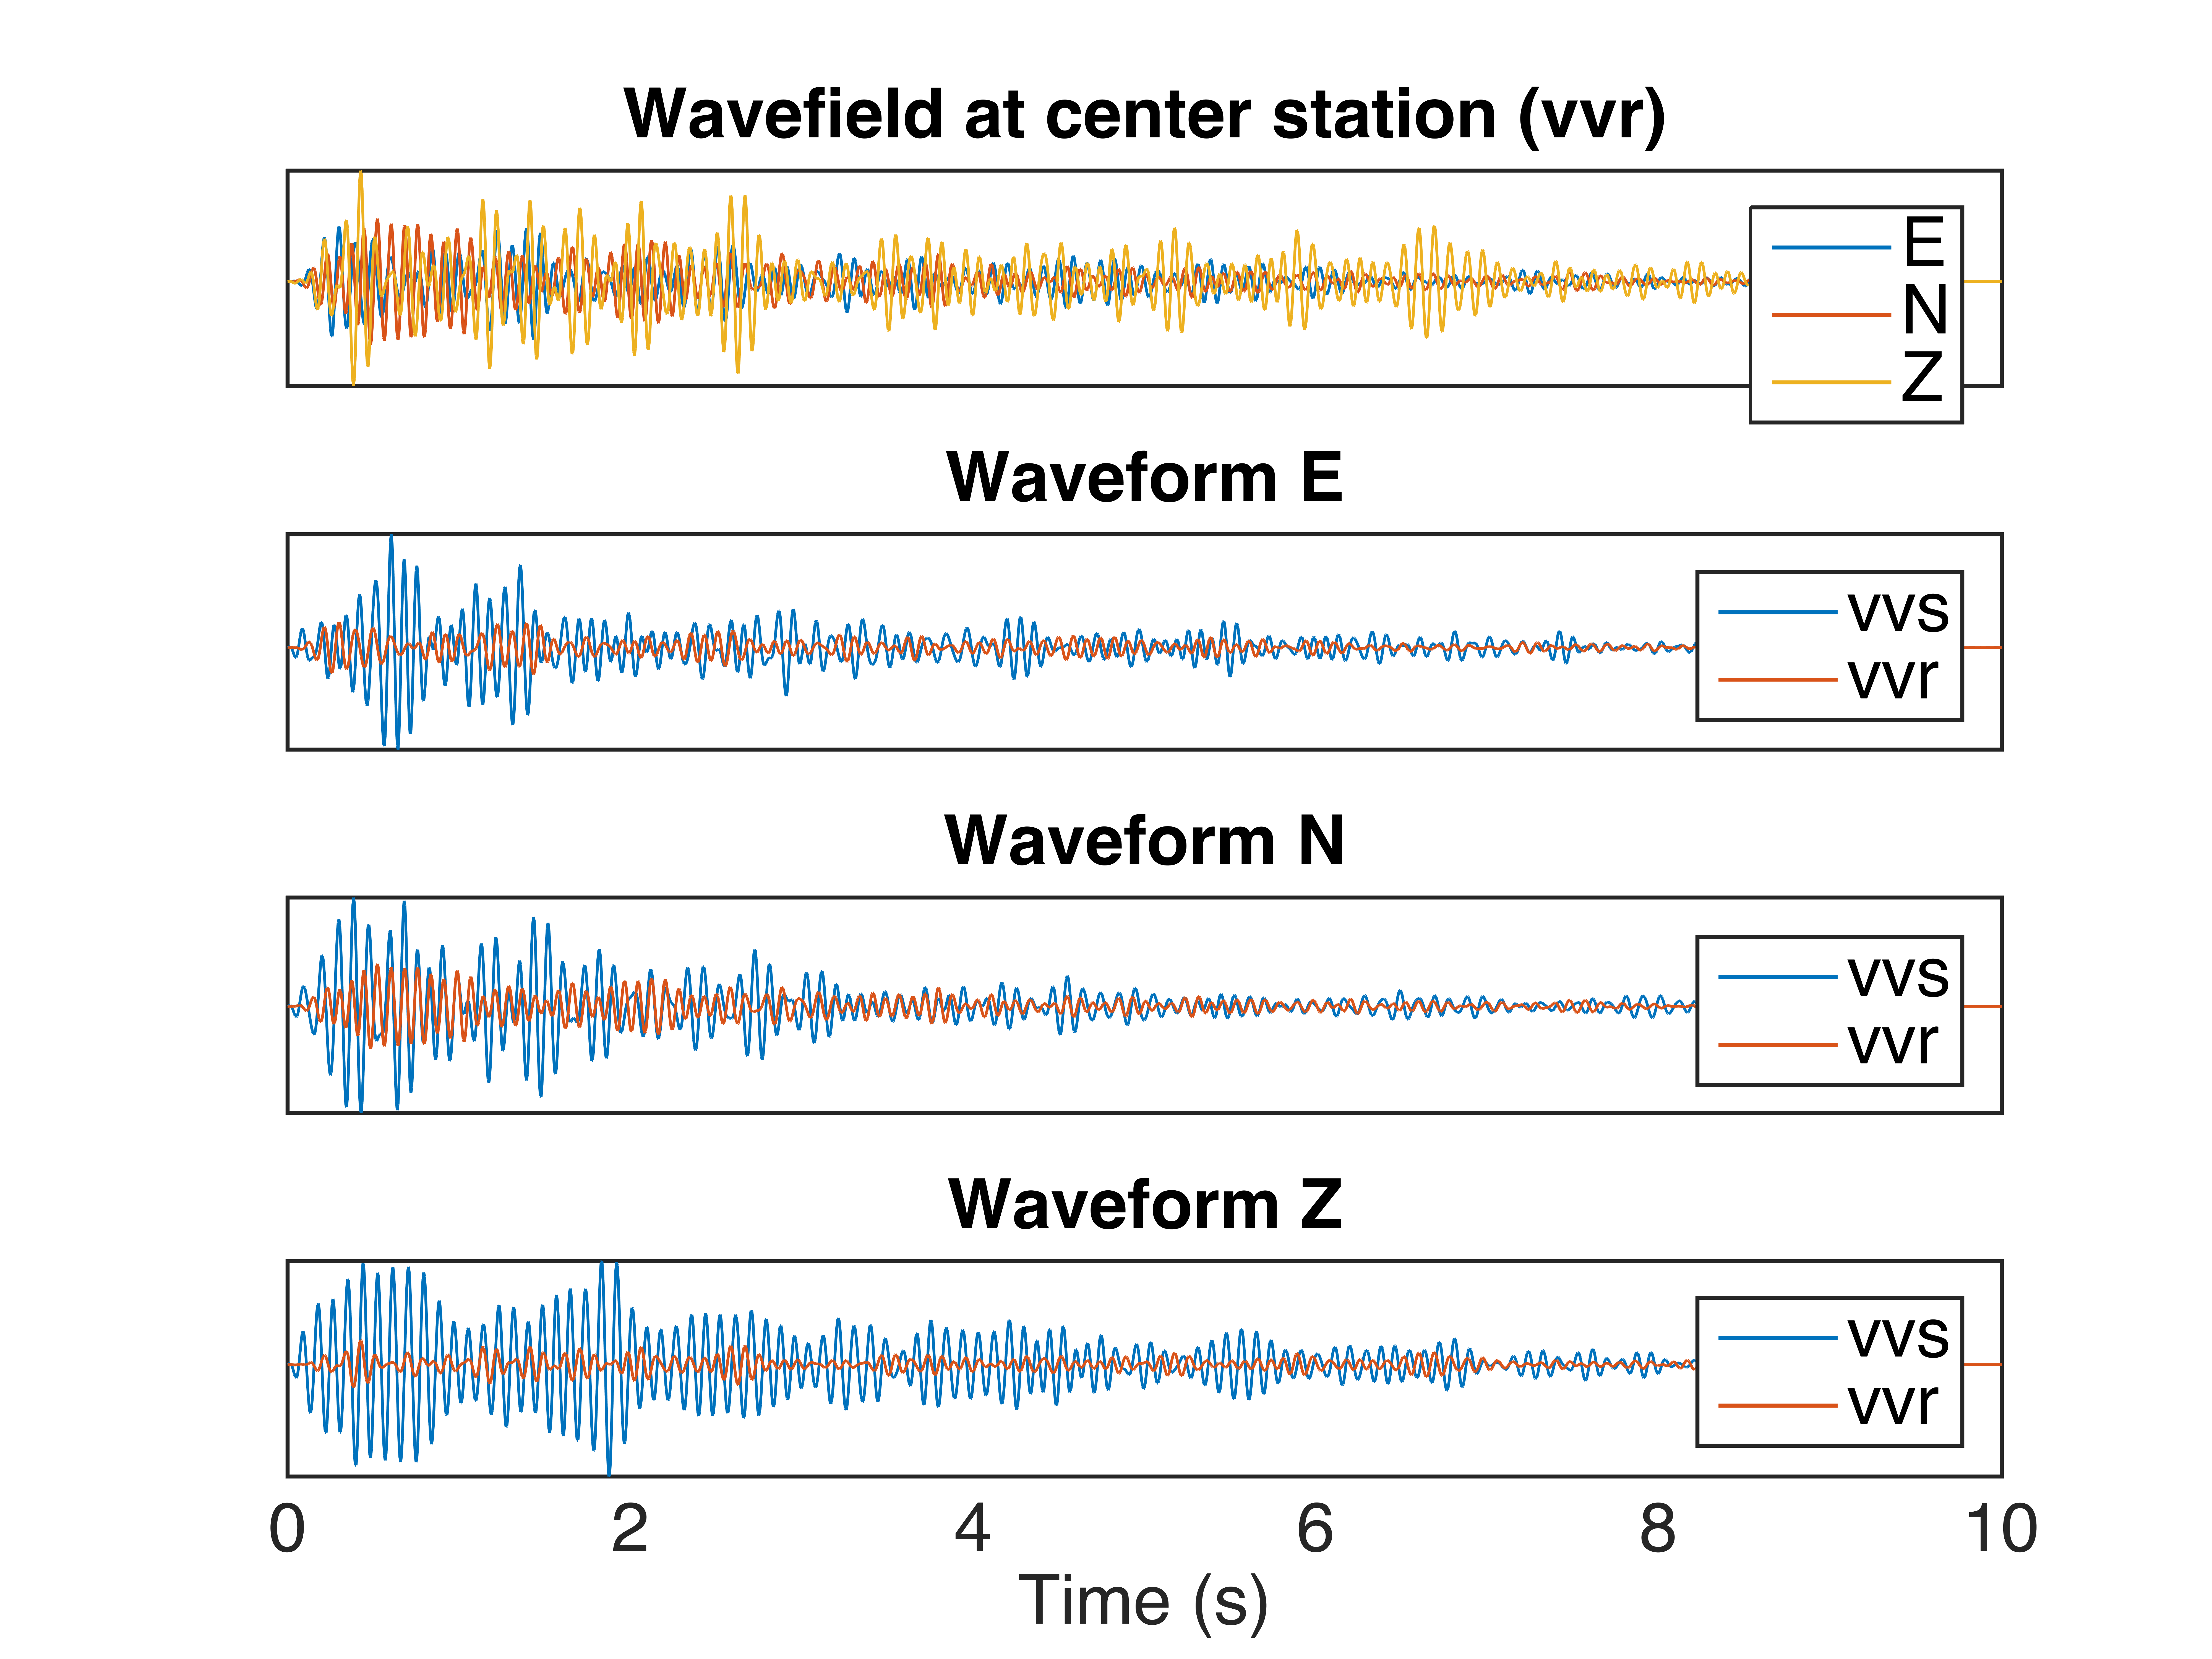
\includegraphics[width=\textwidth]{../pics/C-78-405/vvr.png}
}
%--------------------------------------------------------------------
%            diffusion 1d                                                                                 
%--------------------------------------------------------------------
\frame
{
\centering
{\bf Observations}
}
%--------------------------------------------------------------------
%            diffusion 1d                                                                                 
%--------------------------------------------------------------------
\frame
{
\frametitle{{\bf Interesting}}
\begin{itemize}
\item This method overshoots (or undershoots) values for $v_p$
\item Concavities of $v_p$ are switched
\item Interferometry-inception enhances contrasts in $v_p$
\item Sensitive knobs to turn:
\\~\\
\begin{itemize}
\item Frequencies for bandpass:
\\~\\
data can get aliased and turn into wiggly cones
\\~\\
\item Time windows for xcorrelations:
\\~\\
group dispersion semblance can become skewed and useless
\\~\\
\item Choosing $s_p^o$:
\\~\\
phase velocities can result increasing in frequency
\\~\\
\end{itemize}
\end{itemize}
}
\end{document}

%
%
%----
% frame
%----
\withoutheadline
{
}
\frame
{
\frametitle{stuff}
}
%
%
\begin{columns}
\begin{column}{0.5\textwidth}

\end{column}
\begin{column}{0.5\textwidth} 

\end{column}
\end{columns}
%
%
\includegraphics[height=3cm,trim={0 0 460 0},clip]{soap_film2.jpg} % trim=left bottom right top
%
%
\iffalse
\fi

